
%% bare_jrnl.tex
%% V1.4
%% 2012/12/27
%% by Michael Shell
%% see http://www.michaelshell.org/
%% for current contact information.
%%
%% This is a skeleton file demonstrating the use of IEEEtran.cls
%% (requires IEEEtran.cls version 1.8 or later) with an IEEE journal paper.
%%
%% Support sites:
%% http://www.michaelshell.org/tex/ieeetran/
%% http://www.ctan.org/tex-archive/macros/latex/contrib/IEEEtran/
%% and
%% http://www.ieee.org/



% *** Authors should verify (and, if needed, correct) their LaTeX system  ***
% *** with the testflow diagnostic prior to trusting their LaTeX platform ***
% *** with production work. IEEE's font choices can trigger bugs that do  ***
% *** not appear when using other class files.                            ***
% The testflow support page is at:
% http://www.michaelshell.org/tex/testflow/


%%*************************************************************************
%% Legal Notice:
%% This code is offered as-is without any warranty either expressed or
%% implied; without even the implied warranty of MERCHANTABILITY or
%% FITNESS FOR A PARTICULAR PURPOSE! 
%% User assumes all risk.
%% In no event shall IEEE or any contributor to this code be liable for
%% any damages or losses, including, but not limited to, incidental,
%% consequential, or any other damages, resulting from the use or misuse
%% of any information contained here.
%%
%% All comments are the opinions of their respective authors and are not
%% necessarily endorsed by the IEEE.
%%
%% This work is distributed under the LaTeX Project Public License (LPPL)
%% ( http://www.latex-project.org/ ) version 1.3, and may be freely used,
%% distributed and modified. A copy of the LPPL, version 1.3, is included
%% in the base LaTeX documentation of all distributions of LaTeX released
%% 2003/12/01 or later.
%% Retain all contribution notices and credits.
%% ** Modified files should be clearly indicated as such, including  **
%% ** renaming them and changing author support contact information. **
%%
%% File list of work: IEEEtran.cls, IEEEtran_HOWTO.pdf, bare_adv.tex,
%%                    bare_conf.tex, bare_jrnl.tex, bare_jrnl_compsoc.tex,
%%                    bare_jrnl_transmag.tex
%%*************************************************************************

% Note that the a4paper option is mainly intended so that authors in
% countries using A4 can easily print to A4 and see how their papers will
% look in print - the typesetting of the document will not typically be
% affected with changes in paper size (but the bottom and side margins will).
% Use the testflow package mentioned above to verify correct handling of
% both paper sizes by the user's LaTeX system.
%
% Also note that the "draftcls" or "draftclsnofoot", not "draft", option
% should be used if it is desired that the figures are to be displayed in
% draft mode.
%
\documentclass[journal]{IEEEtran}

\newcommand{\eref}[1]{(\ref{#1})}
\newcommand{\fref}[1]{Fig.~\ref{#1}}
\newcommand{\tref}[1]{Table~\ref{#1}}
\newcommand{\sref}[1]{Section~\ref{#1}}
\newcommand{\aref}[1]{Appendix~\ref{#1}}
\newcommand{\alref}[1]{Algorithm~\ref{#1}}
\newcommand{\unit}[1]{\ensuremath{\, \mathrm{#1}}}
\usepackage{tikz}
\usepackage{balance}
\usepackage{textcomp}
\usepackage{amssymb}
\usepackage{xcolor}
% \definecolor{DarkGreen}{rgb}{0,0.5,0}
% \def\gtick{\textcolor{DarkGreen}{\checkmark}}
\def\gtick{\checkmark}
% \definecolor{DarkRed}{rgb}{0.5,0,0}
% \def\rcross{\textcolor{DarkRed}{x}}
\def\rcross{x}
\usepackage[pdftex]{rotating}

%
% If IEEEtran.cls has not been installed into the LaTeX system files,
% manually specify the path to it like:
% \documentclass[journal]{../sty/IEEEtran}





% Some very useful LaTeX packages include:
% (uncomment the ones you want to load)


% *** MISC UTILITY PACKAGES ***
%
%\usepackage{ifpdf}
% Heiko Oberdiek's ifpdf.sty is very useful if you need conditional
% compilation based on whether the output is pdf or dvi.
% usage:
% \ifpdf
%   % pdf code
% \else
%   % dvi code
% \fi
% The latest version of ifpdf.sty can be obtained from:
% http://www.ctan.org/tex-archive/macros/latex/contrib/oberdiek/
% Also, note that IEEEtran.cls V1.7 and later provides a builtin
% \ifCLASSINFOpdf conditional that works the same way.
% When switching from latex to pdflatex and vice-versa, the compiler may
% have to be run twice to clear warning/error messages.






% *** CITATION PACKAGES ***
%
%\usepackage{cite}
% cite.sty was written by Donald Arseneau
% V1.6 and later of IEEEtran pre-defines the format of the cite.sty package
% \cite{} output to follow that of IEEE. Loading the cite package will
% result in citation numbers being automatically sorted and properly
% "compressed/ranged". e.g., [1], [9], [2], [7], [5], [6] without using
% cite.sty will become [1], [2], [5]--[7], [9] using cite.sty. cite.sty's
% \cite will automatically add leading space, if needed. Use cite.sty's
% noadjust option (cite.sty V3.8 and later) if you want to turn this off
% such as if a citation ever needs to be enclosed in parenthesis.
% cite.sty is already installed on most LaTeX systems. Be sure and use
% version 4.0 (2003-05-27) and later if using hyperref.sty. cite.sty does
% not currently provide for hyperlinked citations.
% The latest version can be obtained at:
% http://www.ctan.org/tex-archive/macros/latex/contrib/cite/
% The documentation is contained in the cite.sty file itself.






% *** GRAPHICS RELATED PACKAGES ***
%
\ifCLASSINFOpdf
  \usepackage[pdftex]{graphicx}
  % declare the path(s) where your graphic files are
  % \graphicspath{{../pdf/}{../jpeg/}}
  \graphicspath{{./figures/}}
  % and their extensions so you won't have to specify these with
  % every instance of \includegraphics
  % \DeclareGraphicsExtensions{.pdf,.jpeg,.png}
  \DeclareGraphicsExtensions{.png}
\else
  % or other class option (dvipsone, dvipdf, if not using dvips). graphicx
  % will default to the driver specified in the system graphics.cfg if no
  % driver is specified.
  % \usepackage[dvips]{graphicx}
  % declare the path(s) where your graphic files are
  % \graphicspath{{../eps/}}
  % and their extensions so you won't have to specify these with
  % every instance of \includegraphics
  % \DeclareGraphicsExtensions{.eps}
\fi
% graphicx was written by David Carlisle and Sebastian Rahtz. It is
% required if you want graphics, photos, etc. graphicx.sty is already
% installed on most LaTeX systems. The latest version and documentation
% can be obtained at: 
% http://www.ctan.org/tex-archive/macros/latex/required/graphics/
% Another good source of documentation is "Using Imported Graphics in
% LaTeX2e" by Keith Reckdahl which can be found at:
% http://www.ctan.org/tex-archive/info/epslatex/
%
% latex, and pdflatex in dvi mode, support graphics in encapsulated
% postscript (.eps) format. pdflatex in pdf mode supports graphics
% in .pdf, .jpeg, .png and .mps (metapost) formats. Users should ensure
% that all non-photo figures use a vector format (.eps, .pdf, .mps) and
% not a bitmapped formats (.jpeg, .png). IEEE frowns on bitmapped formats
% which can result in "jaggedy"/blurry rendering of lines and letters as
% well as large increases in file sizes.
%
% You can find documentation about the pdfTeX application at:
% http://www.tug.org/applications/pdftex





% *** MATH PACKAGES ***
%
\usepackage[cmex10]{amsmath}
% A popular package from the American Mathematical Society that provides
% many useful and powerful commands for dealing with mathematics. If using
% it, be sure to load this package with the cmex10 option to ensure that
% only type 1 fonts will utilized at all point sizes. Without this option,
% it is possible that some math symbols, particularly those within
% footnotes, will be rendered in bitmap form which will result in a
% document that can not be IEEE Xplore compliant!
%
% Also, note that the amsmath package sets \interdisplaylinepenalty to 10000
% thus preventing page breaks from occurring within multiline equations. Use:
\interdisplaylinepenalty=2500
% after loading amsmath to restore such page breaks as IEEEtran.cls normally
% does. amsmath.sty is already installed on most LaTeX systems. The latest
% version and documentation can be obtained at:
% http://www.ctan.org/tex-archive/macros/latex/required/amslatex/math/





% *** SPECIALIZED LIST PACKAGES ***
%
\usepackage{algorithmic}
% algorithmic.sty was written by Peter Williams and Rogerio Brito.
% This package provides an algorithmic environment fo describing algorithms.
% You can use the algorithmic environment in-text or within a figure
% environment to provide for a floating algorithm. Do NOT use the algorithm
% floating environment provided by algorithm.sty (by the same authors) or
% algorithm2e.sty (by Christophe Fiorio) as IEEE does not use dedicated
% algorithm float types and packages that provide these will not provide
% correct IEEE style captions. The latest version and documentation of
% algorithmic.sty can be obtained at:
% http://www.ctan.org/tex-archive/macros/latex/contrib/algorithms/
% There is also a support site at:
% http://algorithms.berlios.de/index.html
% Also of interest may be the (relatively newer and more customizable)
% algorithmicx.sty package by Szasz Janos:
% http://www.ctan.org/tex-archive/macros/latex/contrib/algorithmicx/
\usepackage{framed} % suggested in http://tex.stackexchange.com/questions/65219/how-to-make-a-code-fragment-in-ieeetran-classes
% My own definition:
\newcounter{algorithm}
\newenvironment{algorithmieee}[1]
{\refstepcounter{algorithm}{1} \begin{figure} \textbf{Algorithm \arabic{algorithm}:} \textit{#1} %
\begin{algorithmic}[1]}
{\end{algorithmic}
 \end{figure}}

% Adapted from http://tex.stackexchange.com/questions/40228/ieeetrans-template-requires-not-to-use-algorithm-package
\newsavebox{\ieeealgbox}
\newenvironment{algorithmicieee}[1]
  {\refstepcounter{algorithm}
   \begin{lrbox}{\ieeealgbox}
   \begin{minipage}{\dimexpr\columnwidth-2\fboxsep-2\fboxrule}
   \textbf{Algorithm \arabic{algorithm}:} \textit{#1} \par
   \begin{algorithmic}[1]}
  {\end{algorithmic}
   \end{minipage}
   \end{lrbox}\noindent\fbox{\usebox{\ieeealgbox}}}

% *** ALIGNMENT PACKAGES ***
%
%\usepackage{array}
% Frank Mittelbach's and David Carlisle's array.sty patches and improves
% the standard LaTeX2e array and tabular environments to provide better
% appearance and additional user controls. As the default LaTeX2e table
% generation code is lacking to the point of almost being broken with
% respect to the quality of the end results, all users are strongly
% advised to use an enhanced (at the very least that provided by array.sty)
% set of table tools. array.sty is already installed on most systems. The
% latest version and documentation can be obtained at:
% http://www.ctan.org/tex-archive/macros/latex/required/tools/


% IEEEtran contains the IEEEeqnarray family of commands that can be used to
% generate multiline equations as well as matrices, tables, etc., of high
% quality.




% *** SUBFIGURE PACKAGES ***
%\ifCLASSOPTIONcompsoc
%  \usepackage[caption=false,font=normalsize,labelfont=sf,textfont=sf]{subfig}
%\else
%  \usepackage[caption=false,font=footnotesize]{subfig}
%\fi
% subfig.sty, written by Steven Douglas Cochran, is the modern replacement
% for subfigure.sty, the latter of which is no longer maintained and is
% incompatible with some LaTeX packages including fixltx2e. However,
% subfig.sty requires and automatically loads Axel Sommerfeldt's caption.sty
% which will override IEEEtran.cls' handling of captions and this will result
% in non-IEEE style figure/table captions. To prevent this problem, be sure
% and invoke subfig.sty's "caption=false" package option (available since
% subfig.sty version 1.3, 2005/06/28) as this is will preserve IEEEtran.cls
% handling of captions.
% Note that the Computer Society format requires a larger sans serif font
% than the serif footnote size font used in traditional IEEE formatting
% and thus the need to invoke different subfig.sty package options depending
% on whether compsoc mode has been enabled.
%
% The latest version and documentation of subfig.sty can be obtained at:
% http://www.ctan.org/tex-archive/macros/latex/contrib/subfig/




% *** FLOAT PACKAGES ***
%
%\usepackage{fixltx2e}
% fixltx2e, the successor to the earlier fix2col.sty, was written by
% Frank Mittelbach and David Carlisle. This package corrects a few problems
% in the LaTeX2e kernel, the most notable of which is that in current
% LaTeX2e releases, the ordering of single and double column floats is not
% guaranteed to be preserved. Thus, an unpatched LaTeX2e can allow a
% single column figure to be placed prior to an earlier double column
% figure. The latest version and documentation can be found at:
% http://www.ctan.org/tex-archive/macros/latex/base/


%\usepackage{stfloats}
% stfloats.sty was written by Sigitas Tolusis. This package gives LaTeX2e
% the ability to do double column floats at the bottom of the page as well
% as the top. (e.g., "\begin{figure*}[!b]" is not normally possible in
% LaTeX2e). It also provides a command:
%\fnbelowfloat
% to enable the placement of footnotes below bottom floats (the standard
% LaTeX2e kernel puts them above bottom floats). This is an invasive package
% which rewrites many portions of the LaTeX2e float routines. It may not work
% with other packages that modify the LaTeX2e float routines. The latest
% version and documentation can be obtained at:
% http://www.ctan.org/tex-archive/macros/latex/contrib/sttools/
% Do not use the stfloats baselinefloat ability as IEEE does not allow
% \baselineskip to stretch. Authors submitting work to the IEEE should note
% that IEEE rarely uses double column equations and that authors should try
% to avoid such use. Do not be tempted to use the cuted.sty or midfloat.sty
% packages (also by Sigitas Tolusis) as IEEE does not format its papers in
% such ways.
% Do not attempt to use stfloats with fixltx2e as they are incompatible.
% Instead, use Morten Hogholm'a dblfloatfix which combines the features
% of both fixltx2e and stfloats:
%
% \usepackage{dblfloatfix}
% The latest version can be found at:
% http://www.ctan.org/tex-archive/macros/latex/contrib/dblfloatfix/




%\ifCLASSOPTIONcaptionsoff
%  \usepackage[nomarkers]{endfloat}
% \let\MYoriglatexcaption\caption
% \renewcommand{\caption}[2][\relax]{\MYoriglatexcaption[#2]{#2}}
%\fi
% endfloat.sty was written by James Darrell McCauley, Jeff Goldberg and 
% Axel Sommerfeldt. This package may be useful when used in conjunction with 
% IEEEtran.cls'  captionsoff option. Some IEEE journals/societies require that
% submissions have lists of figures/tables at the end of the paper and that
% figures/tables without any captions are placed on a page by themselves at
% the end of the document. If needed, the draftcls IEEEtran class option or
% \CLASSINPUTbaselinestretch interface can be used to increase the line
% spacing as well. Be sure and use the nomarkers option of endfloat to
% prevent endfloat from "marking" where the figures would have been placed
% in the text. The two hack lines of code above are a slight modification of
% that suggested by in the endfloat docs (section 8.4.1) to ensure that
% the full captions always appear in the list of figures/tables - even if
% the user used the short optional argument of \caption[]{}.
% IEEE papers do not typically make use of \caption[]'s optional argument,
% so this should not be an issue. A similar trick can be used to disable
% captions of packages such as subfig.sty that lack options to turn off
% the subcaptions:
% For subfig.sty:
% \let\MYorigsubfloat\subfloat
% \renewcommand{\subfloat}[2][\relax]{\MYorigsubfloat[]{#2}}
% However, the above trick will not work if both optional arguments of
% the \subfloat command are used. Furthermore, there needs to be a
% description of each subfigure *somewhere* and endfloat does not add
% subfigure captions to its list of figures. Thus, the best approach is to
% avoid the use of subfigure captions (many IEEE journals avoid them anyway)
% and instead reference/explain all the subfigures within the main caption.
% The latest version of endfloat.sty and its documentation can obtained at:
% http://www.ctan.org/tex-archive/macros/latex/contrib/endfloat/
%
% The IEEEtran \ifCLASSOPTIONcaptionsoff conditional can also be used
% later in the document, say, to conditionally put the References on a 
% page by themselves.




% *** PDF, URL AND HYPERLINK PACKAGES ***
%
%\usepackage{url}
% url.sty was written by Donald Arseneau. It provides better support for
% handling and breaking URLs. url.sty is already installed on most LaTeX
% systems. The latest version and documentation can be obtained at:
% http://www.ctan.org/tex-archive/macros/latex/contrib/url/
% Basically, \url{my_url_here}.




% *** Do not adjust lengths that control margins, column widths, etc. ***
% *** Do not use packages that alter fonts (such as pslatex).         ***
% There should be no need to do such things with IEEEtran.cls V1.6 and later.
% (Unless specifically asked to do so by the journal or conference you plan
% to submit to, of course. )


% correct bad hyphenation here
\hyphenation{op-tical net-works semi-conduc-tor}

% ++++ Used temporarily to make comments between authors
\newcommand{\comment}[1]{{\color{red} #1}}
\usepackage[normalem]{ulem}
\newcommand{\commentErrase}[1]{\comment{\sout{#1}}}

\begin{document}
%
% paper title
% can use linebreaks \\ within to get better formatting as desired
% Do not put math or special symbols in the title.
% could we change the title to this? What do you think? I wanted to get the modular idea in there.
\title{A Multi-Modal Model of Object Deformation under Robotic Pushing
%A Multi-Modal Model for Prediction and Classification of Object Deformation during Robotic Manipulation
}
%
%
% author names and IEEE memberships
% note positions of commas and nonbreaking spaces ( ~ ) LaTeX will not break
% a structure at a ~ so this keeps an author's name from being broken across
% two lines.
% use \thanks{} to gain access to the first footnote area
% a separate \thanks must be used for each paragraph as LaTeX2e's \thanks
% was not built to handle multiple paragraphs
%

\author{Veronica E.~Arriola-Rios,
        Jeremy~L.~Wyatt \thanks{V.E. Arriola-Rios is with Facultad de Ciencias, UNAM, Mexico, e-mail: v.arriola@ciencias.unam.mx}
        \thanks{J.L. Wyatt is with the University of Birmingham, Edgbaston, Birmingham, B15 2TT, UK. e-mail: jeremy.l.wyatt@gmail.com }}%
% <-this % stops a space
%\thanks{J.L. Wyatt is with the University of Birmingham, Edgbaston, Birmingham, B15 2TT, UK. e-mail: jeremy.l.wyatt@gmail.com }% <-this % stops a space
%\thanks{Manuscript received April 19, 2005; revised December 27, 2012.}}

% note the % following the last \IEEEmembership and also \thanks - 
% these prevent an unwanted space from occurring between the last author name
% and the end of the author line. i.e., if you had this:
% 
% \author{....lastname \thanks{...} \thanks{...} }
%                     ^------------^------------^----Do not want these spaces!
%
% a space would be appended to the last name and could cause every name on that
% line to be shifted left slightly. This is one of those "LaTeX things". For
% instance, "\textbf{A} \textbf{B}" will typeset as "A B" not "AB". To get
% "AB" then you have to do: "\textbf{A}\textbf{B}"
% \thanks is no different in this regard, so shield the last } of each \thanks
% that ends a line with a % and do not let a space in before the next \thanks.
% Spaces after \IEEEmembership other than the last one are OK (and needed) as
% you are supposed to have spaces between the names. For what it is worth,
% this is a minor point as most people would not even notice if the said evil
% space somehow managed to creep in.



% The paper headers
\markboth{IEEE CDS}%
{Arriola-Rios and Wyatt: A Multi-Modal Model of Object Deformation for Robotic Pushing}
% The only time the second header will appear is for the odd numbered pages
% after the title page when using the twoside option.
% 
% *** Note that you probably will NOT want to include the author's ***
% *** name in the headers of peer review papers.                   ***
% You can use \ifCLASSOPTIONpeerreview for conditional compilation here if
% you desire.




% If you want to put a publisher's ID mark on the page you can do it like
% this:
%\IEEEpubid{0000--0000/00\$00.00~\copyright~2012 IEEE}
% Remember, if you use this you must call \IEEEpubidadjcol in the second
% column for its text to clear the IEEEpubid mark.

% use for special paper notices
%\IEEEspecialpapernotice{(Invited Paper)}




% make the title area
\maketitle

% As a general rule, do not put math, special symbols or citations
% in the abstract or keywords.
\begin{abstract}
In this paper we present a multi-modal framework for \comment{offline} learning of generative models of object deformation under robotic pushing. The model is multi-modal in that it is based on integrating force and visual information. The framework consists of several sub-models that are independently \comment{calibrated} from the same data. These component models can be sequenced to provide many-step prediction and classification. When presented with a test example--a robot finger pushing a deformable object made of an unidentified, but previously learned, material--the predictions of modules for different materials are compared so as to classify the unknown material. Our approach, which consists of \comment{offline learning and combination of} multiple models, goes beyond previous techniques by enabling i) predictions over many steps, ii) learning of plastic and elastic deformation from real data, iii) prediction of forces experienced by the robot, iv) classification of materials from both force and visual data, v) prediction of object behaviour after contact by the robot terminates.  While previous work on deformable object behaviour in robotics has offered one or two of these features none has offered a way to achieve them all, and none has offered classification from a generative model. We do so through separately learned models which can be combined in different ways for different purposes.
\end{abstract}

% Note that keywords are not normally used for peerreview papers.
\begin{IEEEkeywords}
deformable objects, prediction, classification, learning.
\end{IEEEkeywords}

% For peer review papers, you can put extra information on the cover
% page as needed:
% \ifCLASSOPTIONpeerreview
% \begin{center} \bfseries EDICS Category: 3-BBND \end{center}
% \fi
%
% For peerreview papers, this IEEEtran command inserts a page break and
% creates the second title. It will be ignored for other modes.
\IEEEpeerreviewmaketitle



\section{Introduction}
% The very first letter is a 2 line initial drop letter followed
% by the rest of the first word in caps.
% 
% form to use if the first word consists of a single letter:
% \IEEEPARstart{A}{demo} file is ....
% 
% form to use if you need the single drop letter followed by
% normal text (unknown if ever used by IEEE):
% \IEEEPARstart{A}{}demo file is ....
% 
% Some journals put the first two words in caps:
% \IEEEPARstart{T}{his demo} file is ....
% 
% Here we have the typical use of a "T" for an initial drop letter
% and "HIS" in caps to complete the first word.
\IEEEPARstart{A} major challenge in robot manipulation is to plan actions with objects so as to deform them into new shapes. Most objects that are manipulated by animals in natural environments are deformable, including objects that are elastic, plastic, breakable, tearable, and spreadable. The work reported here is based on the premise that in order to plan manipulations of deformable objects, the sensorimotor contingencies governing object deformation are required. A sensorimotor contingency is simply defined as the relationship between the robot's actions and the resultant changes in its observations. Different materials (here, elastic and plastic materials) have different sensorimotor contingencies. The main hypothesis is that predictive models of these sensorimotor contingencies can be learned from data. The predictions of a learned model can be fed back into itself, so as to predict an object's deformation behaviour over many time steps. These learned models can then be used to make the predictions required for planning manipulation.

There are various models of deformation used in engineering, such as finite element models, but these typically require careful optimisation by hand, and cannot run in real time. In graphics there are many methods used for generating qualitatively plausible simulations of deformable objects, but these are not easy to fit to real data. \comment{In contrast, robots must learn model parameters from data, in reasonable amounts of training time. This includes learning from the limited sensing typically available, such as training data gathered from a specific view(s) of an object, and force-torque monitoring only at contact points.} Thus, tackling the prediction problem in robotics adds additional difficulties to an already challenging problem. \comment{In this paper we address some of these---we learn from real visual and force-torque data---while simplifying others---we set a convenient fixed viewing location and perform off-line rather than on-line learning.}

%\begin{figure}[!t]
%\centering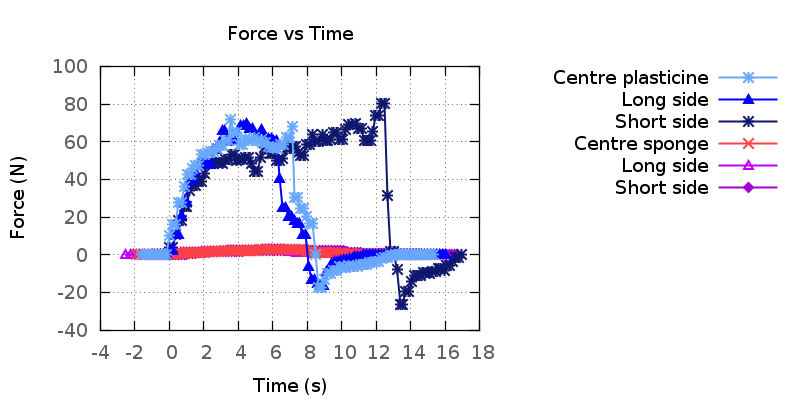
\includegraphics[width=3.5in]{arrio17.png}
%\caption{Force information acquired while working with a block of sponge (elastic) and a piece of plasticine (plastic).  Notice the difference in magnitude between the force used with the sponge and the plasticine.}
%\label{fig:forceElasticPlastic}
%\end{figure}

Previous work on learning sensorimotor contingencies for deformable objects in robotics has been limited. Table~\ref{t:advances} summarises the features of the major efforts to date. In each case some abilities are missing: either models cannot be learned from data; or only address one type of deformation (e.g. elastic); or cannot perform classification; or cannot predict the forces felt; or cannot predict what will happen when the robot loses contact with the object (will it retain or recover from the deformation?). In this paper we present an approach for solving all these problems. Although our framework requires two separate learned models, they are combined into a single machine for prediction of the behaviour of deformable material. In a second machine, multiple copies of this predictor can be compared to an actual outcome deformation, so as to classify the material.

\comment{There are two novel technical contributions. First, we show how the learning problem can be decomposed into two separate learning problems, one for predicting forces from finger motions, and one for predicting object deformations from forces. Both models are generative, and we show how to learn each from data. Second, we show how to use these learned generative models not only to predict deformation, but also to classify an unidentified material. To limit the scope of the paper we develop this framework using offline learning methods. We do not address the issue of online learning \cite{worgotter09,antonelli14}, leaving this for future work.}

 %This behaviour is described in \alref{alg:overall}.

%\begin{figure}
% \begin{algorithmicieee}{Overall Behaviour}\label{alg:overall}
% {\small
% \STATE \textbf{Training Phase:}
% \FORALL {training materials:}
%   \FORALL {finger commands (push down, push up)}
%     \STATE The controler gives the command.
%     \WHILE {the command is executed}
%       \STATE The F/T sensor module records the reaction force.
%       \FORALL {candidate regresion curves}
%         \STATE The F/T sensor module adjusts the curve.
%       \ENDFOR
%       \STATE The visual system tracks and records the modifications of the shape from a 2D camera.
%     \ENDWHILE
%     \STATE The F/T sensor module records a discontinuity in the regresion curve.
%   \ENDFOR
%   \STATE The F/T sensor module returns the best regresion curve as Model B.
%   \STATE The learning algorith for the mass-spring model proposes candidate parameters.
%   \FORALL{frames of captured information}
%     \FORALL{sets of candidate parameters}
%       \STATE Evaluate how similar the mass-spring simulation is to the real object.
%     \ENDFOR
%   \ENDFOR
%   \STATE The values of the best set of parameters is adopted as Model A.
% \ENDFOR
% \STATE \textbf{Simulation Phase:}
% \WHILE{the finger penetrates the material}
%   \STATE Use Model B to predict the reaction force given the distance traversed after contact with the material.
%   \STATE Use this force to run the simulation with Model A.
%   \STATE Model A predicts the shape the material should have.
% \ENDWHILE
% \STATE \textbf{Classification Phase:}
% \FORALL{frames of captured information}
%  \FORALL{previously trained materials}
%    \STATE Run simulation and evaluate similitude
%  \ENDFOR
% \ENDFOR
% \STATE Return material with the highest score.}
% \end{algorithmicieee}
%\caption{Overall algorithmic structure of the system.}
%\end{figure}

\comment{These technical contributions} enable us to learn models of sensorimotor contingencies, and then to use these as components to build different machines. This approach enables i) predictions over many steps, ii) learning of plastic and elastic deformation from real data, iii) prediction of forces experienced by the robot, iv) classification of materials from either or both force and visual data, v) prediction of object behaviour after contact by the robot is removed. In the rest of the paper we present related work (Section~\ref{sec:background}); give an overview of the framework (Section~\ref{sec:model_overview}); describe the two component models in detail (Section~\ref{sec:model}); describe how the model parameters are learned from real data for the shape prediction model (Section~\ref{sec:learning}) and for the force prediction model (Section~\ref{sec:forces}); report experiments on prediction and classification with elastic and plastic objects (Section~\ref{sec:experiments}); and finish with a short discussion (Section~\ref{sec:discussion}).

% needed in second column of first page if using \IEEEpubid
%\IEEEpubidadjcol




% An example of a floating figure using the graphicx package.
% Note that \label must occur AFTER (or within) \caption.
% For figures, \caption should occur after the \includegraphics.
% Note that IEEEtran v1.7 and later has special internal code that
% is designed to preserve the operation of \label within \caption
% even when the captionsoff option is in effect. However, because
% of issues like this, it may be the safest practice to put all your
% \label just after \caption rather than within \caption{}.
%
% Reminder: the "draftcls" or "draftclsnofoot", not "draft", class
% option should be used if it is desired that the figures are to be
% displayed while in draft mode.
%
%\begin{figure}[!t]
%\centering
%\includegraphics[width=2.5in]{myfigure}
% where an .eps filename suffix will be assumed under latex, 
% and a .pdf suffix will be assumed for pdflatex; or what has been declared
% via \DeclareGraphicsExtensions.
%\caption{Simulation Results.}
%\label{fig_sim}
%\end{figure}

% Note that IEEE typically puts floats only at the top, even when this
% results in a large percentage of a column being occupied by floats.


% An example of a double column floating figure using two subfigures.
% (The subfig.sty package must be loaded for this to work.)
% The subfigure \label commands are set within each subfloat command,
% and the \label for the overall figure must come after \caption.
% \hfil is used as a separator to get equal spacing.
% Watch out that the combined width of all the subfigures on a 
% line do not exceed the text width or a line break will occur.
%
%\begin{figure*}[!t]
%\centering
%\subfloat[Case I]{\includegraphics[width=2.5in]{box}%
%\label{fig_first_case}}
%\hfil
%\subfloat[Case II]{\includegraphics[width=2.5in]{box}%
%\label{fig_second_case}}
%\caption{Simulation results.}
%\label{fig_sim}
%\end{figure*}
%
% Note that often IEEE papers with subfigures do not employ subfigure
% captions (using the optional argument to \subfloat[]), but instead will
% reference/describe all of them (a), (b), etc., within the main caption.


% An example of a floating table. Note that, for IEEE style tables, the 
% \caption command should come BEFORE the table. Table text will default to
% \footnotesize as IEEE normally uses this smaller font for tables.
% The \label must come after \caption as always.
%
%\begin{table}[!t]
%% increase table row spacing, adjust to taste
%\renewcommand{\arraystretch}{1.3}
% if using array.sty, it might be a good idea to tweak the value of
% \extrarowheight as needed to properly center the text within the cells
%\caption{An Example of a Table}
%\label{table_example}
%\centering
%% Some packages, such as MDW tools, offer better commands for making tables
%% than the plain LaTeX2e tabular which is used here.
%\begin{tabular}{|c||c|}
%\hline
%One & Two\\
%\hline
%Three & Four\\
%\hline
%\end{tabular}
%\end{table}


% Note that IEEE does not put floats in the very first column - or typically
% anywhere on the first page for that matter. Also, in-text middle ("here")
% positioning is not used. Most IEEE journals use top floats exclusively.
% Note that, LaTeX2e, unlike IEEE journals, places footnotes above bottom
% floats. This can be corrected via the \fnbelowfloat command of the
% stfloats package.

% \section{Model Overview}
% \label{sec:model_overview}
% 
% As has been mentioned above there are several choices made in our modeling approach. The key choice is that the models are generative, which means that the models can be used to generate predicted sequences of behaviour. The specific approach taken here separates the predictive model out into components in two ways (see Figure~\ref{fig:system}). First we decompose models according to the modality of the information. In this case it is important to note that deformation has a particular causal structure related to the modes of sensing that are most easily employed. The forces and deformations can be measured separately, using force-torque and visual sensors respectively. The sensed forces are the cause of the observed deformation, and this can be exploited by sequencing the models by mode. Thus our approach can be seen as a sensorimotor contingency in which two contigencies are sequenced to produce an overall prediction. The input to the first predictor is the planned motion of the robot (or the joint torques), and this predictor predicts the resulting sequence of contact forces. The second predictor takes this sequence of forces as input and predicts a deformation sequence. Both models must be conditioned on the material and the object. This is where we decompose the model space in the second way, by specialising models to particular material and object combinations. This follows the principle of modular motor learning \cite{KopickiICRA11,haruno2001mosaic}, where prediction and control is specialised into many modules, each of which covers a relatively small portion of the input space, such as an object or material type. Thus we aim to acquire many specialist models of different deformable objects rather than a very few rather general models. The specific model forms we choose here could be replaced while retaining the overall scheme. In this paper we implement the scheme using a regression approach to force prediction, and we follow several other authors in employing a mass-spring system with learnable parameters for the deformation prediction.
% 
% In each case the models can be run in two modes, prediction and classification. In prediction mode the models make predictions based on a sequence of robot finger positions. To create the prediction for time $t+1$ the previous predicted state at time $t$ is required: thus the predictions are recursive. This enables predictions over arbitrarily long time periods, but makes learning a good predictor challenging. In filtering mode the predictions of different models are compared to the actual outcomes, and this is used to classify the object as being one of the modular models in the set of models. Since the model is multi-modal we can compare both force and deformation data to the corresponding model predictions. 
% 
% The training of the model is performed offline using ground truthed data. %The overall algorithm is given in \alref{alg:overall}.
% For clarity the algorithm is given in three phases: training, simulation (i.e. the prediction phase), and classification (i.e. matching prediction to new data). In testing the model new data is used, where this is typically new deformation actions on an object of known material and approximate shape. Having given an overview of the model we now relate our approach to those in the literature, before proceeding to describe the details of the spring-mass model of deformation (Section~\ref{sec:model}), and then the regression model of contact forces (Section~\ref{sec:forces}).

\section{Background}
\label{sec:background}

It is known that the human motor system uses predictive (or forward) models of the effects that motor actions have on sensory state \cite{flanagan03,flanagan06,johansson92}. These are believed to be particularly important for dexterous manipulation. In robotics, prediction of physical interaction is a well studied but incompletely solved problem. There is a large body of work on the effects of pushing on rigid objects. This includes physics based models \cite{lynch_mechanics_1992,peshkin_motion_1988,mason_mechanics_2001} and learning approaches \cite{montesano08,moldovan12,fitzpatrick_learning_2003,kroemer2014,Stoytchev_affordances_2008,mericli2014, scholz2010combining,kopicki-etal-icra11,kopickiwyatt16,belter2014iros}. These predictive models have many applications, including visual tracking \cite{morwald2011icra, duff2011icra, pham2015capturing} and push planning \cite{stillman08ijrr,Dogar_2010,lynchmason96,zitoetal-iros12,Cosgun2011}.

There is much less work in robotics on predicting the behaviour of deformable objects under manipulation. This paper focuses on learning to predict what happens when an elastic or plastic object is pushed by a robot finger. These predictions include the response forces and the deformations of the object's shape over many future steps. The predictive models can be used to classify materials, even when the interactions (e.g. the contact point) are novel. Although there is a large body of work on deformable object tracking, some of which makes use of forces, models and predictions to improve tracking accuracy \cite{Chan1994, Greminger2008, Alkkiomaki2009}, those predictions are typically used only for the next frame and can not be used for robotic planning, where predictions must be made many steps into the future \cite{Cretu2012}.  Others like \cite{Malassiotis1998, Cremers2006} make use of templates or make assumptions about the shape of the objects that would not work with highly deformable objects like plasticine.  There is also an abundant literature in industrial robotics for modelling 1D and 2D materials (e.g. string, hair, metallic sheet and textile), but there is little research about predicting the deformation of 3D deformable objects \cite{Khalil2010review}. We now review the most closely related work to that presented here.

\begin{table}[t]
  %\renewcommand{\arraystretch}{1.3}
  \caption{Advances over previous work}\label{t:advances}
  \begin{tabular}{lccccccccc}
  %\hline\hline \\ [-1.5ex]
  \hline \\ [-1.5ex]
 & \begin{sideways}\textbf{Model type}\end{sideways} & \begin{sideways}\textbf{Learned from GT}\end{sideways} & \begin{sideways}\textbf{GT=Real data}\end{sideways} & \begin{sideways}\textbf{Prediction of Shape} \end{sideways} & \begin{sideways}\textbf{Prediction of Forces}\end{sideways} & \begin{sideways}\textbf{Actuator Retrieval} \end{sideways} & \begin{sideways}\textbf{Elastic}\end{sideways} & \begin{sideways}\textbf{Plastic}\end{sideways} & \begin{sideways}\textbf{Classification}\end{sideways} \\
 \hline\hline \\ [-1.5ex]
  Howard & MS & \gtick  & \gtick  & \rcross & \gtick & \rcross & \gtick & \rcross & \rcross\\
Teschner & MS & \rcross & \rcross & \gtick & \rcross & \gtick & \gtick & \gtick & \rcross \\
  Morris & MS & \gtick  & \rcross & \gtick & \rcross & \rcross & \gtick & \rcross & \rcross \\
  Frank & FEM & \gtick  & \gtick & \gtick & \rcross & QSA & \gtick & \rcross & \rcross \\
  This work & MS & \gtick  & \gtick & \gtick & \gtick & \gtick & \gtick & \gtick & \gtick \\
         & + &&&&&&&&\\
         & Regression &&&&&&&& \\
 %[-1.5ex] \\ \hline\hline \\ [-1.5ex]
 [-1.5ex] \\ \hline \\ [-1.5ex]
 \end{tabular}
 *MS = \textit{Mass-spring}\\
 *QSA = \textit{Quasi-Static Assumption}
\end{table}

First, Howard and Bekey \cite{Howard2000} address robotic grasping and lifting of viscoelastic objects.  Their model of the material can predict a net amount of deformation given the applied forces, but does not evaluate details of the deformed shape.   This model is inspired by the crystalline structure of atoms in solids.  The space lattice of the crystal is approximated by a particle system where elements with mass are connected by springs and dampers, thus representing the attraction and repulsion between atoms \emph{in equilibrium} with a damped mass-spring system.  The masses are calculated by measuring the force required to lift the object without sliding.  The deformation and damping coefficients are estimated as functions of:
\begin{itemize}
 \item the force applied while pushing against the material with two robot arms in opposite directions and,
 \item the global displacement and velocity vectors resulting from adding the displacements and velocities of all particles.
\end{itemize}
The estimated values of the mass, deformability and damping coefficients are used as the input to a neural network that outputs the minimum necessary force to lift the object without sliding.  This function is used to compliantly adjust the force during an interaction.  However, they do not evaluate the quality of the overall shape prediction, and use only the final values of the prediction after the system has stabilised; that is, they do not evaluate the predictions during the dynamic phase.

%\begin{figure}[!t]
%\centering
%\setlength\fboxsep{0pt}    % padding
%\setlength\fboxrule{0.5pt} % line width
%\fbox{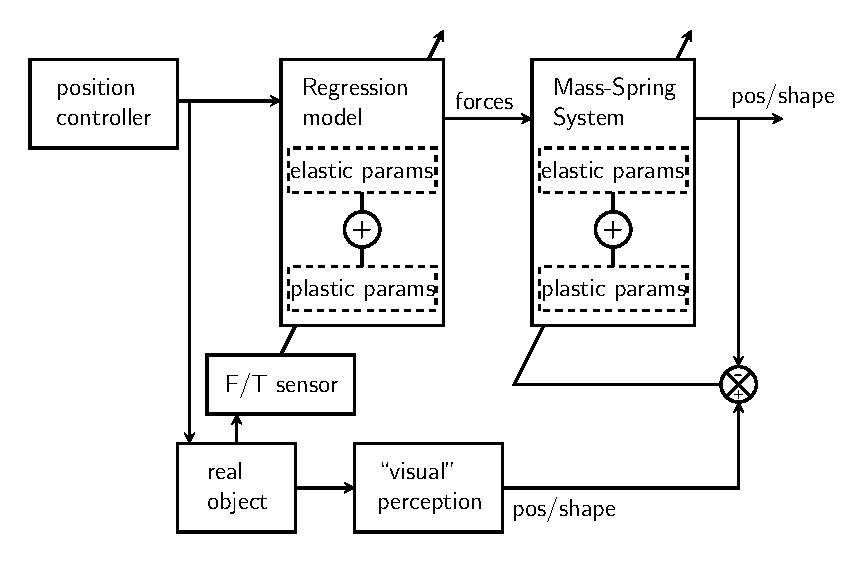
\includegraphics[width=3.5in]{arrio3.pdf}}
%\caption{During training time, the system learns to predict the object's shape and reaction forces from real world data.}
%\label{fig:system}
%\end{figure}

%%%
%%% TODO: Text
%%%
% \begin{figure}[!t]
% \centering
% \setlength\fboxsep{0pt}    % padding
% \setlength\fboxrule{0.5pt} % line width
% \fbox{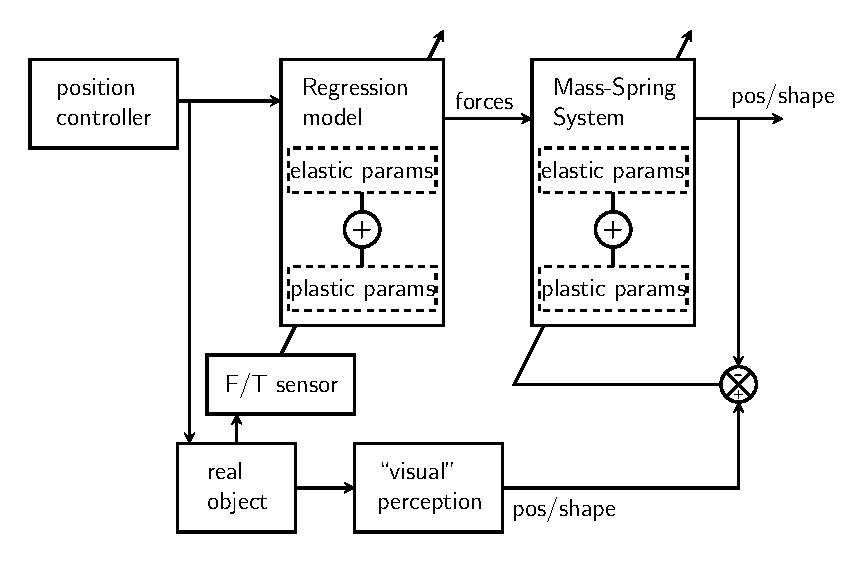
\includegraphics{arrio3}}
% \caption{The system learns to predict the object's shape and reaction forces from real world data.}
% \label{fig:system_old}
% \end{figure}

Teschner et al.\ \cite{Teschner2004} proposed an enhanced 3D mass-spring model, in which constraints are expressed as potential energy terms.  These terms encode the tendency of springs to recover their length (with damping), of triangular faces of a mesh to recover their area and of tetrahedrons to recover their volume.  He sketches the inclusion of plastic deformation.  Morris and Salisbury \cite{Morris2008} developed a method to calibrate Teschner's model automatically with respect to a \comment{finite element model (FEM)}.  The  search begins with a uniform random sampling of possible values for the elasticity constants, which are latter modified using adaptive simulated annealing to minimize the difference between the deformations in the FEM mesh and those in the mass-spring mesh.  However, they only compare the steady states and do not include plastic deformations.  We extend this work, by replacing the FEM model with force and 2D visual data gathered from real materials.  Furthermore, we analyse the quality of the predictions while the deformations take place.

Frank et al.\ \cite{Frank2010} use a force sensor and a bumblebee stereo camera to measure the Young modulus and the Poisson ratio of unknown deformable objects.  By assuming a homogeneous material, they propose candidate values for these constitutive parameters and simulate the expected behaviour of the object with a FEM method.  The volume of the prediction is compared with a 3D reconstruction of the 3D surface of the object.  A gradient descent search is used to minimize the difference.  Once the parameters are selected, a collision detection algorithm informs the model of the position of the actuator, thus implying the amount of local deformation.  The FEM simulation provides estimates for the global deformation and response forces.  However, a quasi-static assumption is made and a detailed study of the dynamic process is not offered.\footnote{With the quasi-static assumption a small force is applied and a state of equilibrium is reached before a new force is applied.  Therefore the deformation process is approximated 
by a series of states of equilibrium.}  The resulting model is applied to estimating costs of robotic navigation around deformable objects \cite{Frank2011}. 

The advances of our work with respect to these related approaches is summarised in \tref{t:advances}.

\begin{figure}[!t]
\centering
%\setlength\fboxsep{0.5pt}    % padding
%\setlength\fboxrule{0.5pt} % line width
%\fbox{
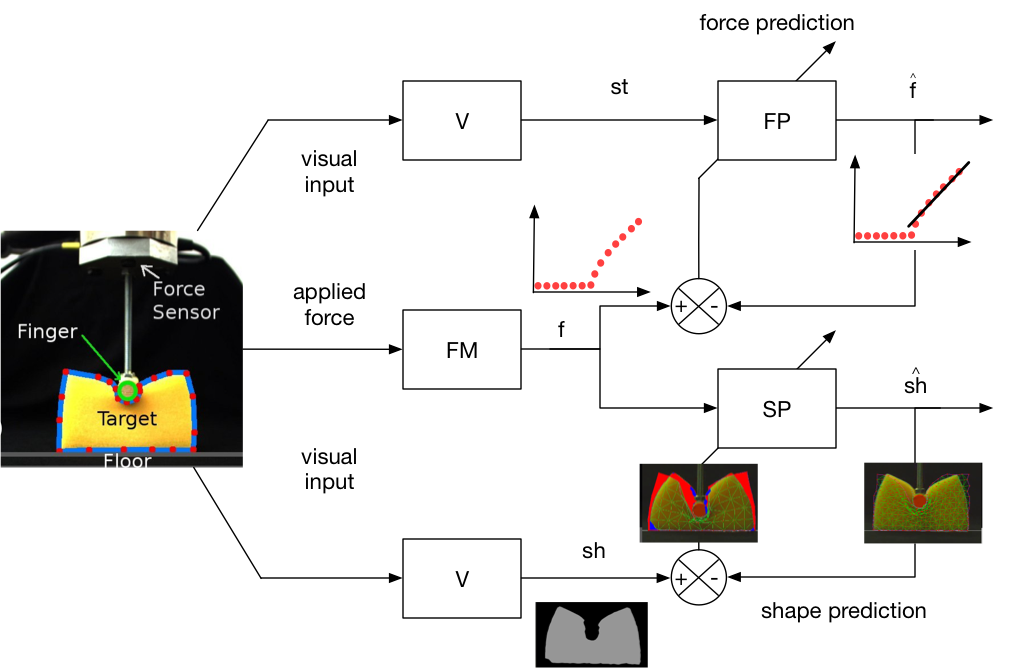
\includegraphics[width=3.5in]{figures/learning.png}%}
\caption{\comment{The visual tracking and force measurement system subserves the offline learning system. The offline learning (or calibration) method comprises two learned models of sensorimotor contingencies.} Both are learned from the same data. The first (FP) learns to predict the force experienced for some motion and material. The second (SP) predicts the deformation of the object given the applied force. The strain $st$ is calculated directly from the interpenetration of the finger into the object. This can be calculated by vision (V) or from the planned motion of the finger.}
\label{fig:learning}
\end{figure}

Other interesting work includes that of Conti et al.\ \cite{Conti2003} which introduced six-degree of freedom macroscopic elastic spheres described by mass, inertial and volumetric properties that are used to approximate the volume of deformable objects. The open source project Chai3D includes an implementation of this model. The spheres are placed along the skeleton of the object and are connected together with elastic links which model elongation, flexion and torsion properties. Each vertex of the surface mesh is attached to the nearest sphere or link with a damped spring.  In \cite{Burion2008}, Burion and Baur, collaborated with Conti's group to automatically calibrate this model using particle filters.  Again, there is no analysis of the dynamics and no real objects are used.  Furthermore, this model is more adequate for objects that deform around fixed joints.

Finally, Cretu et al. \cite{Cretu2012}, used growing neural gas networks to learn to predictively track the deformation of objects.  Even though they managed to make predictions about the deformation of the overall shape of the object, under previously unseen sets of forces, their predictions were evaluated only for the next frame.

Additionally, there is a vast literature on modeling of deformable shapes and deformation processes \cite{Gibson1997, McInerney1996, Montagnat2001, Moore2007review, Nealen2006review}, particularly within the area of computer graphics.  However, these types of models have not been successfully applied to robotics tasks beyond what is presented above.

%\subsection{Predicting the Shape}
%Contribution: we analyse the dynamic behaviour of the predictions for several frames.
%\subsection{Predicting the Force}
%Physics based models are used to predict reaction forces (surgery simulators).
%Contribution: we learn to predict with a linear regression model.  Also calibrated automatically.

\section{Model Overview}
\label{sec:model_overview}

\comment{The framework consists of four separate systems: a visual tracking and force measurement system, an offline learning (or model calibration) system, a prediction system, and a classification system. 

Visual tracking and force measurement both serve the learning system (Figure~\ref{fig:learning}). The visual analysis is not a contribution of the paper, any method that provides accurate tracking of the outline of the deformed object would suffice. We employ a Canny edge detector, filtering out irrelevant edges using the colour of the manipulated object. Then we fit the outline and track using a linear snake. This is also used to initialise the mesh for the spring mass system.}

The learning system is depicted in Figure~\ref{fig:learning}. This enables learning of sensorimotor contingencies from real robot data. Learning of the force prediction (FP) model relies on comparing the predicted $\hat{f}$ and the experienced $f$ forces at the finger tip, as measured by a force-torque sensor (FM). Learning of the shape prediction (SP) model relies on comparing the predicted deformation $\hat{sh}$ with the actual deformation $sh$ measured by visual tracking (V).

\comment{In machine learning there is division between discriminative and generative models. Discriminative models are powerful for classification, but cannot be used to regenerate the data, or to generate new imagined data. In our application this would mean we could not predict deformations, only being able to classify materials directly based on their deformations. Instead, following others, we use a generative model. But we show how this can be used not just for prediction, but also for material classification. Thus a generative model is appealing because it allows us to solve both the prediction and classification problems.}

The two learned generative models, FP and SP, can be sequenced to create a single, multi-modal predictor (Figure~\ref{fig:prediction}). This combined model takes a planned motion of the finger, and predicts the resulting forces that will be experienced at the contact points. It then uses both the planned positions and predicted forces to predict the resulting object deformations. Typically, a sequence of planned finger positions will be known. In prediction mode the models make predictions based on this sequence. To create the prediction for time $t+1$ the previous predicted state at time $t$ is required: thus the predictions are recursive. This enables predictions over arbitrarily long time periods, but makes learning a good predictor challenging.

\begin{figure}[t]
\centering
%\setlength\fboxsep{0pt}    % padding
%\setlength\fboxrule{0.5pt} % line width
%\fbox{
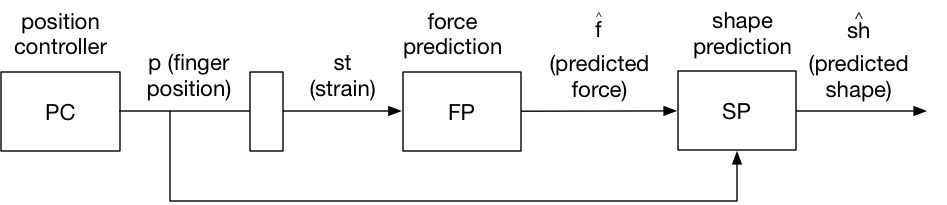
\includegraphics[width=3.5in]{figures/prediction}%}
\caption{The two learned models can be sequenced, so as to predict an object's shape and reaction forces when the robot finger will push in a particular way. The predicted shape is fed back on itself so as to predict over many steps for a planned sequence of finger motion. PC is the position controller for the robot, which outputs each planned finger position $p$ at each time. This is used to calculate the strain $st$ from the interpenetration using a fixed function, as well as providing an input to the shape predictor (SP).}
\label{fig:prediction}
\end{figure}

\begin{figure*}[!t]
\centering
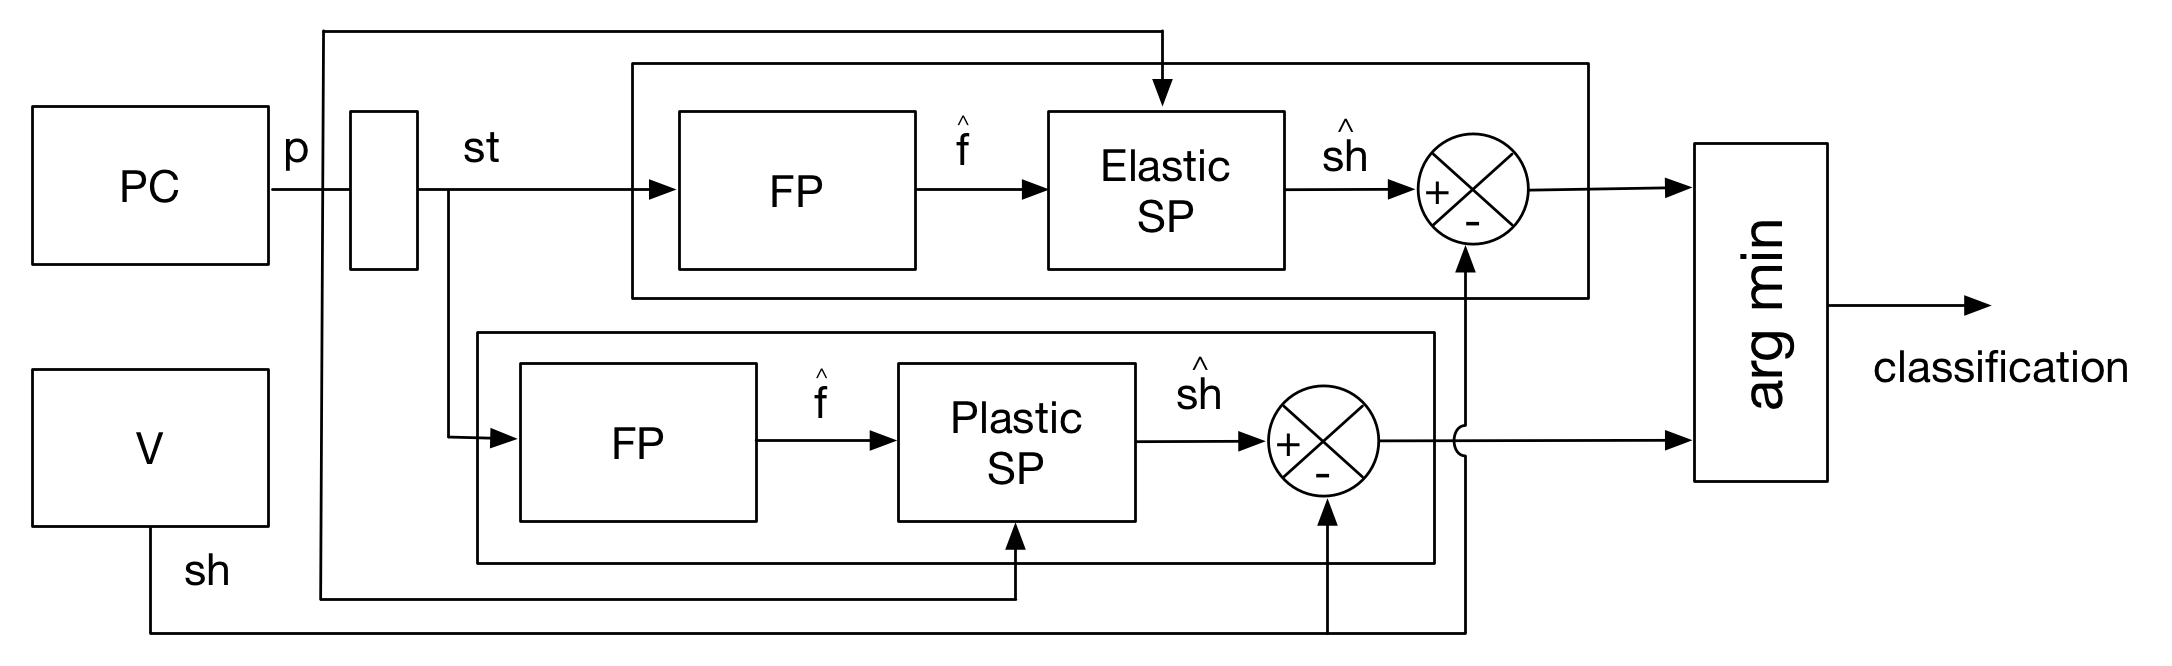
\includegraphics[width=0.8\textwidth]{figures/classification}
\caption{Prediction sequences for several predictors--each of which has been learned for a different material--can be compared against real data. The most accurate predictor at any one moment gives the classification for the material type. The notation is explained in the text.}
\label{fig:classification}
\end{figure*}

The third system is for material classification (Figure~\ref{fig:classification}). This simply comprises multiple copies of the prediction systems, one for each type of material that an unknown object might be made of. The predictors each make many-step predictions. At each step a classification is made, based on which predictor has made the better prediction of the shape at that step.

In summary, this way of learning and using models involves several choices. First, the learned models are generative. Second, our approach can be seen as one in which two contingencies are learned separately, and then sequenced to produce an overall prediction. Third, although here we only compare two material models for prediction, the scheme follows the principle of modular motor learning \cite{kopickiwyatt16,haruno2001mosaic}, where prediction and control is specialised into many modules, each of which covers a relatively small portion of the input space, such as an object or material type. Thus the aim of a generalised version of our scheme will be to acquire many specialist models of different deformable objects rather than a very few rather general models. The specific model forms we choose here could be replaced while retaining the overall scheme. In this paper, we implement the scheme using a regression approach to force prediction, and we follow several other authors in employing a mass-spring system with learnable parameters for the deformation prediction.

%As has been mentioned above, there are several choices made in our modeling approach. The key choice is that the models are generative, which means that the models can be used to generate predicted sequences of behaviour. The specific approach taken here separates the predictive model out into components in two ways (see Figure~\ref{fig:system}). First we decompose models according to the modality of the information. In this case it is important to note that deformation has a particular causal structure related to the modes of sensing that are most easily employed. The forces and deformations can be measured separately, using force-torque and visual sensors respectively. The sensed forces are the cause of the observed deformation, and this can be exploited by sequencing the models by mode. Thus our approach can be seen as a sensorimotor contingency in which two contingencies are sequenced to produce an overall prediction. The input to the first predictor is the planned motion of the robot (or the joint torques), and this predictor predicts the resulting sequence of contact forces. The second predictor takes this sequence of forces as input and predicts a deformation sequence. Both models must be conditioned on the material and the object. This is where we decompose the model space in the second way, by specialising models to particular material and object combinations. This follows the principle of modular motor learning \cite{kopickiwyatt16,haruno2001mosaic}, where prediction and control is specialised into many modules, each of which covers a relatively small portion of the input space, such as an object or material type. Thus the aim of a generalised version of our scheme is to acquire many specialist models of different deformable objects rather than a very few rather general models. The specific model forms we choose here could be replaced while retaining the overall scheme. In this paper we implement the scheme using a regression approach to force prediction, and we follow several other authors in employing a mass-spring system with learnable parameters for the deformation prediction.

%In each case the resulting learned models can be run in two modes, prediction and classification. In prediction mode the models make predictions based on a sequence of robot finger positions. To create the prediction for time $t+1$ the previous predicted state at time $t$ is required: thus the predictions are recursive. This enables predictions over arbitrarily long time periods, but makes learning a good predictor challenging. In filtering mode the predictions of different models are compared to the actual outcomes, and this is used to classify the object as being one of the modular models in the set of models. Since the model is multi-modal we can compare both force and deformation data to the corresponding model predictions.

%The training of the model is performed offline using ground truthed data. %The overall algorithm is given in \alref{alg:overall}.
For clarity, the algorithm is described in exactly these phases: training, simulation (i.e. the prediction phase), and classification. In empirically evaluating the model new data was used, acquired from new finger pushes. We now proceed to describe first the visual analysis and force measurement, the force predictor (FP), which is a regression model (Section~\ref{sec:forces}), and then the shape predictor SP (Section~\ref{sec:model}), which is based on a mass-spring system.

\section{Visual Analysis}
\label{sec:vision}

Although the visual analysis is not an original contribution of the paper, it is necessary to track the shape of the object as it deforms. This tracking is performed on the two training movies to provide training data for the shape predictor (SP). For the test movies the system only requires visual analysis of the first frame to initialise the predictors. The test movies are analysed for each frame, but only for experimental evaluation purposes. We now give details of the visual analysis method.

\subsection{Tracking to Provide Ground Truth}
\begin{figure}[!t]
 \begin{algorithmicieee}{Regularised Linear Spline}\label{alg:regularise}
 \STATE Let $L$ be a linear spline representing the contour of a $2D$ shape, and $L_i$ the $i^{th}$ control point in a cyclic order.
 \FORALL {$L_i$ in $L$}
 \IF {$dist(L_i,L_{i-1}) > max\_distance$}
  \STATE Insert $midpoint(L_i,L_{i-1})$ after $L_i$
 \ELSIF {$dist(L_i,L_{i-1}) < min\_distance$}
  \STATE erase $L_i$
 \ELSIF {$angle(L_{i-1},L_i,L_{i+1}) < min\_angle$}
  \STATE erase $L_i$
 \ENDIF
 \ENDFOR
\end{algorithmicieee}
\caption{Algorithm used to regularise the number of elements of a linear spline, in accordance with the level of detail required.}
\end{figure}
 The contour of the deformable object is used to obtain the ground truth for the training phase, which is the area enclosed by the contour. Since we only require a tracking algorithm which is good enough to evaluate the predictions of the mass-spring system, a very simple one was used.  Geometrically, the contour is represented by a polygon with hundreds of sides, which can also be called a \textit{linear spline} \cite{Menet1991}. The vertices of the polygon work as control points which can be moved to adjust the polygon to the shape of the object as it gets deformed.  \comment{We call our algorithm for tracking a \emph{linear snake}, because}  this implementation is inspired by the theory of active contours, however it works with a much simpler and faster, but less accurate, algorithm, instead of minimizing a global energy.  \comment{This causes some shadowed corners of the material to be missed at some frames, but as \fref{fig:scene}(b) at its bottom left shows, these errors are not significant in comparison to the errors made by the mass-spring model.} This is explained below.  The tracking of the deformable target in the ground truth has two stages:
 \begin{figure}[t]
\centering
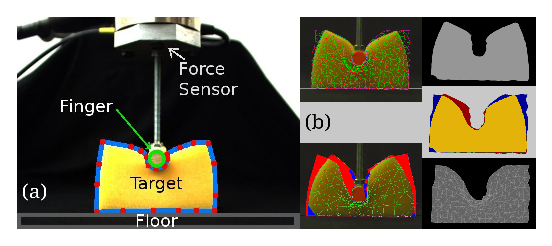
\includegraphics[width=88mm]{arrio2}
\caption{(a) Experimental set up.  A robot finger pushes a block of deformable material sitting on a table.  A camera registers the events of the plane where the main deformations take place.  (b) Evaluation function.  Left top: Mesh over real block of material.  Left bottom: The typical error of the model vs. the ground truth (red) and the typical error of the tracker (blue).  Right top: tracked ground data.  Middle: TP in yellow, FP in blue, FN in red and TN in gray.  Bottom: simulated mesh. }
\label{fig:scene}
\end{figure}

\begin{enumerate}
 \item The target object is segmented from the environment.  The Canny algorithm is used to extract the edges of the image.  Since the object of interest has a distinctive colour, \comment{its characteristic hue range is extracted from the area enclosed by the initial contour.  Then} the hue of the pixels on every edge are used to keep only edges that could belong to it.  If the average hue of the pixels on an edge falls outside the calibrated range, the edge is eliminated.
 \item The internal representation of its contour, the linear snake, is adapted to its new shape.  The algorithm assumes that no occlusions take place and that the contour does not bend over itself.
\end{enumerate}
For the first frame, the snake is initialised as a rectangle around the target. This rectangle fragments itself into smaller pieces. Each new vertex adheres itself to the closest point on an edge, as reached by growing rings of pixels around its current position, up to a certain threshold distance [\fref{fig:scene}(a)].  If there is no edge within that area, the control point remains where it is. This criterion was selected to make the representation more robust against edges that are easier to detect on some frames than in others.  Once the edge reappears, the control point adapts itself again.  Also, the distance between two consecutive control points is kept within the interval $[min\_distance, max\_distance]$ and two adjacent edges do not form angles smaller than $min\_angle$.  See \alref{alg:regularise}.  This allows the snake to adapt very quickly to the complexity of the contour it represents.

\section{Learning to predict forces}
\label{sec:forces}

It is possible to learn the force predictor (FP), by using information from the stress-strain diagram obtained from the data set of measured positions and forces.  This diagram is obtained from the video recorded by the visual system of the robot and the forces recorded by the sensor located at the wrist.  When the readings of the force sensor start to increase and the figer collides with the block of material, the point of zero deformation is identified.  From here on, the displacement of the finger is considered equivalent to the amount of deformation in the material.  Even though this method is not as rigorous as an engineering test, the estimation is good enough for robot manipulation of common materials.

The stress strain curves in [\fref{fig:sstrain}] are approximated by segmented regression curves.  Several candidates are proposed using the least squares technique and the best are chosen as follows.  Since there is only one independent variable the equations for adjusting a line are straightforward:

\begin{align}
 y & = mx + y_0 + Error \\
 m & = \dfrac{n\sum x_i y_i-\sum x_i \sum y_i}{n \sum x_i^2 -(\sum x_i)^2} \\
 y_0 & = \dfrac{\sum y_i}{n} - y_0 \dfrac{\sum x_i}{n} \displaybreak[0] \\
 Error & = \sum(y_i - (mx_i+y0))^2
\end{align}
Where $y$ is the dependent variable, $x$ the independent one, $m$ is the slope of the line, and $y_0$ the $y$ intercept.  To adjust logarithmic curves a change of variable is used.  Before computing the line, the natural logarithm of the independent variable is calculated, that is: $x'_i = \ln(x_i)$.  In this case, the final equation will be of the form: $y = m \ln x + y_0$.  It would be possible to add other types of curves, but these were enough for the materials covered.

For automatic calibration of the force prediction model for the pushing (as opposed to retraction) phase both families of lines (logarithmic curves and straight lines) are considered.  To determine the points of discontinuity between segments, each family is evaluated incrementally. The candidate line for a particular family is obtained by fitting a growing subset of data points and calculating the fitting error.  We begin with a small number of points (e.g. five). To detect the discontinuity new points are added until the corresponding normalized error increases beyond a threshold value.  This marks the point of discontiuity. Having discovered one best parameterized line for each family, the two resulting candidates are compared. We select the type of curve that covers more points in a single segment.  This model is used to predict the forces for the mass-spring simulation \fref{fig:diagram} and \fref{fig:sstrain}.


\section{A Mass-Spring Model of Deformation}
The shape predictor (SP) is based on a mass-spring model of deformation.  A mass-spring model is a very well established abstraction, commonly used to simulate the behaviour of certain types of deformable objects.  As a physics based model, once its parameters are acquired, its behaviour is determined by the evolution of a set of differential equations.  Therefore, by offering a method to automatically calibrate those parameters, this model can make long term predictions about the behaviour of deformable objects, under previously unseen interactions, if only the externally applied forces are known.  The range of validity of these predictions greatly depends on the quality of the calibration, but also on the suitability of the mass-spring model as a model of the particular object.  For this reason, there are variations that address specific issues, like \cite{Bourguignon2000} and \cite{Teschner2004}.  In this work, we focus on the machinery required to achieve this automatic calibration of a physics based model and its integration into a system that exploits it to solve prediction and classification tasks.  We emphasize that the physics based model could be easily substituted by another equivalent model.  For example, the same machine will work if another type of mass-spring model is used, or a FEM model, even though numerical results will differ to some extent.  For these experiments we chose to use a slightly modified version of the mass-spring model proposed by Teschner in \cite{Teschner2004}.

%This work makes use of the ability of a mass-spring model to predict the shape of a deformable object given its shape at time $t$ and the forces acting on it.  The parameters, that attune this generic model to a particular object, will be obtained through machine learning, and that procedure will be explained in \sref{sec:learning}, since it is independent of the model itself.  Also the forces required as inputs by this mass-spring model will be learned by another module, so that the entire system will require only the initial shape of the object, and the command to be executed, to be able to predict the future behaviour of the object and sensed feedback force.  This section explains the details of the mass-spring model we used.

In a simple mass-spring model, the shape of an object is approximated by a uniform geometric mesh, usually made of triangles (2D) or tetrahedrons (3D).  At every vertex $i$ in the mesh, an ideal particle with no volume, but with mass $m_i$, is located, and is known as a \textit{mass particle}.  The edges between vertices roughly model the interactions between particles, which attract each other up to a certain critical distance, but repel each other if they become closer, therefore maintaining the cohesion of the solid, while avoiding the collapse of the material on itself.  The simplest model associates a linear spring with each edge, as if those forces would occur only between connected neighbours.  The resting state of the solid corresponds to a configuration of the masses and springs where the sum of all forces acting over each particle is zero, and they are said to be in equilibrium.

When one or more particles are displaced from their equilibirum positions, the forces that tend to restore an elastic body to its original shape are modeled by the forces of springs (along the edges of the mesh) that try to recover their original length).  These forces act upon the particles modifying their positions in time.  Traditionally, the relationship between the position of the particle $p_i$ and those forces $F$ obeys the second law of Newton:
\begin{align}
F = m \dfrac{\partial \vec{p}}{\partial t} \label{eq:newton}
\end{align}
where $t$ is time.  However, it is possible to deviate from this equation if we need to model a different behaviour. %are interested in is numerical accuracy, as it will be done here.

The above equation is a second order differential equation, which is continuous by definition.  In order to perform a computer simulation we need to obtain the position $p$ of all vertices as a function of time $p(t)$ using this equation.  A numerical method is selected to approximate a solution \cite{Nealen2006review}.  Time is discretized in intervals of length $h$, positions and forces at discrete past times are used to estimate the new positions at time $t + h$, according to an integration scheme which must be selected.  The fact that the values of the forces remain constant in this approximation, for the whole interval $h$ (also know as \textit{time step}), introduces errors which can be severe.  For this reason, computer simulations may add procedures that help to alleviate these effects.  

To simulate the effect of an external actuator (like the finger of the robot) interacting with the deformable object, external forces $F_{ext}$ acting on vertices of the mesh must be added to \eref{eq:newton}:
\begin{align}
F + F_{ext} = m \dfrac{\partial \vec{p}}{\partial t}
\end{align}
Another option could be to induce response forces by displacing vertices from their position of equilibrium.


\label{sec:model}
\subsection{Elastic Deformation}

\begin{figure}[t]
\centering
%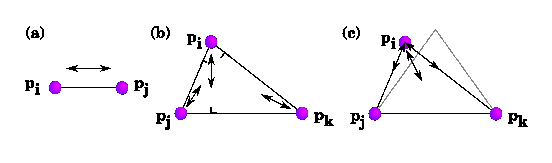
\includegraphics[width=2.5in]{arrio1}
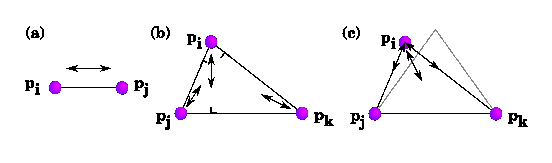
\includegraphics[width=88mm]{arrio1}
\caption{Spring Forces. Recovery of: (a) Length, forces act along the spring.  (b) Area, forces act along the heights of the triangles. (c) Angle, masses slide trying to restore the angle.}
\label{fig:forces}
\end{figure}

The mass-spring model proposed by Teschner et al.\ in \cite{Teschner2004}, which is explained below, was reduced to a 2D model, so that the predictions could be compared with 2D images of the deformable object.  The main idea being that an agent can make rough real time predictions of what it can see and touch and use those predictions to solve various tasks, like classification or grasping.  Here, the surface of the deformable object is approximated by a regular triangular mesh of unitary masses and springs.  \comment{Since the location of the masses and direction of the springs will bias the deformation response of the object, it is important to distribute the masses uniformly and place the springs with a symetric arrangement for an isotropic material.  This placement can be done with an algorithm that takes into account the symmetries of the object at the begining of the experiment.  If the material gets permanently deformed a properly calibrated physics based model, like the one we propose here, will produce an adequate new arrangement from which new interactions can be studied.}

The potential energy terms for the preservation of length with damping and preservation of area were included in our system exactly as they were defined by Teschner.  To compensate for the lack of a term for preservation of volume, which tends to prevent distortions of the graph in the original model, we derived a new term for the preservation of the angles in every triangle.  The relevant equations are presented in the following paragraphs, while detailed derivations can be found in \cite{Arriola2013thesis}.

Teschner defined a generalized version of the simple mass-spring model by using the concept of \emph{constraint}.  He makes use of different constraints to model the tendency of an object to recover several of its attributes. For every desired constraint $C(\vec{p}_1,...,\vec{p}_{n})$ acting over $n$ vertices, a potential energy $E$ is defined.  When the value of the constraint is zero, the potential energy is zero as well.  When the constraint is not satisfied, the potential energy increases.  This behaviour is obtained through the following definition for the energy:
\begin{align}
 E(\vec{p}_1,...,\vec{p}_{n}) & = \frac{1}{2}kC(\vec{p}_1,...,\vec{p}_{n})^2, \label{eq:EConstraint}
\end{align}
where $k$ is a proportionality constant and $p_i$ is the position of particle $i$.

In order to reduce the energy of the system when a constraint is not satisfied, the force $\vec{F}^i$ acting on the $i^{th}$ mass particle is defined as the negative gradient of this potential energy with respect to the position of the particle $\vec{p}_i$ \eref{eq:EForce}.
\begin{align}
 \vec{F}^i(\vec{p}_1,...,\vec{p}_{n}) & = -\frac{\partial}{\partial \vec{p}_i}E = -kC\frac{\partial C}{\partial \vec{p}_i}. \label{eq:EForce}
\end{align}
Given the oscillatory nature of these equations, when using constraints that model the behaviour of springs, damping can be introduced to stop the oscillations.  This is modelled with a force acting in the opposite direction to the velocity of the affected particles, thus slowing down motion.  Teschner wrote this as a function of the constraints as well \cite{Teschner2004}:
\begin{align}
 \label{eq:Fdamping}
 \vec{F}^i&(\vec{p}_1,...,\vec{p}_{n},\vec{v}_1,...,\vec{v}_{n}) = \nonumber \\
    &\left( -kC-k_d\sum_{1 \le j \le n} \dfrac{\partial C}{\partial \vec{p}_j}\vec{v}_j \right)
 \dfrac{\partial C}{\partial \vec{p}_i},
\end{align}
where $\vec{v}_j = \frac{\partial \vec{p}_j}{\partial t}$ is the velocity of the $j^{th}$ particle connected to $i$, when the constraint acts on $n$ particles.

\subsubsection{Preservation of Length}
The constraint for the potential energy is given by:
\begin{equation}
 C = \dfrac{|\vec{p}_j-\vec{p}_i|-D_0}{D_0}, \label{eq:clength}
\end{equation}
where $\vec{p}_i$ and $\vec{p}_j$ are connected by a spring and $D_0$ is the rest length of that spring.  The force derived from this constraint pulls the masses in the direction of the spring that joins them [\fref{fig:forces}(a)].  Teschner normalised the value dividing by $D_0$ to make the elasticity constants scale independent \cite{Teschner2004}.  Morris \cite{Morris2008} omitted that in his final equations for the force.  Here we use the normalised force $\vec{F}^i_D$ \eref{eq:FDlength}, which has the effect that, if we obtain a good set of parameters for a certain mesh of high resolution, the same set can be used for a mesh of lesser resolution that preserves the same type of symmetries.  Details about the final form of this and following equations are in \aref{ap:formulas}.

\subsubsection{Preservation of Area}
This constraint is applied per triangle in the mesh.  Since Teschner and Morris
found that the use of damping for the preservation of areas does not significantly improve the stability of the simulation, it is not included here either.  Therefore the force $\vec{F}^i_A$ is derived from the constraint and \eref{eq:EForce}: 
\begin{align}
 C &= \frac{\frac{1}{2}|(\vec{p}_j-\vec{p}_i)\times(\vec{p}_k-\vec{p}_i)|-A_0}{A_0}
\end{align}
where $A_0$ is the initial area of the triangle and $k_A$ the proportionality constant.

\subsubsection{Preservation of Angles}
The previous terms can not do anything to restore the mesh if triangles get flipped during deformation.  For this reason we included a new term that enforces the preservation of the original angles of the triangles, \comment{which is not a valid state since the mesh models the surface of a 3D object}.  [\fref{fig:forces}(c)] gives an idea of how these forces look.  Here the energy depends on the difference \comment{%\sout{of the angles between adjacent edges.} 
between the current angle, between adjacent edges, and the angle between them at the equilibrium position.} Energy is given by\footnote{It was also considered to multiply $E_\varphi$ by the lengths of the edges, but it hasn't improved the performance of the model.}:
\begin{align}
 E_\varphi(\varphi) & = \frac{1}{2}k_\varphi(\varphi - \varphi_0)^2 \\
 \varphi(p_i,p_j,p_k) & = \arccos \left( \dfrac{(p_j - p_i) \cdot (p_k - p_i)}{ \left\| p_j - p_i \right\| \left\|p_k - p_i \right\|} \right)^2 \nonumber
\end{align}

where $\varphi$ is the angle between adjacent edges, $E_\varphi$ is the energy associated with changes in the angle, $k_\varphi$ is the corresponding stiffness constant, and the $p_i$s are the Cartesian coordinates of the mass particles.

The force emerging from this term is a linear combination of the vectors along the edges that form the angle of interest, acting in the direction of the gradient.  It tends to restore the angles in the most efficient way, but does not take the original size into account [\fref{fig:forces}(c)].  Therefore, it helps to recover a similar triangle, but it may produce tiny or very big triangles if it is not accompanied by some of the other terms that tend to restore the original dimensions, in addition to the angles.

\vspace*{1em}
The terms for the preservation of length and angle model elastic deformations.  Even though the preservation of area by itself would allow some plasticity, it is still necessary to incorporate permanent deformations in the rest lengths of the springs, to stop the triangles of the mesh from trying to recover their original shape.

\subsection{Plastic Deformation}
\begin{figure}
 \begin{algorithmicieee}{Plastic Deformation of an Edge}\label{alg:deformEdge}
\STATE Let $l$ be the length of the edge at time $t+h$, after an integration step where new positions of its vertices $p_i(t+h)$ where calculated. And $max\_\alpha$ the maximum proportional permanent deformation being allowed.
 \IF {$\alpha > max\_\alpha$}
  \STATE $l_0 \gets l$
 \ELSE
  \STATE $l_0 \gets (1.0 - \alpha) D_0$
 \ENDIF
 \STATE $elastic\_deformation \gets \frac{l_0 - l}{D_0}$
 \IF {$elastic\_deformation > yield$}
  \STATE $\alpha \gets \alpha + creep * elastic\_deformation$
  \IF {$\alpha > max\_\alpha$}
   \STATE $\alpha \gets max\_\alpha$
  \ENDIF
 \ENDIF
 \end{algorithmicieee}
\caption{Algorithm to calculate the permanent deformation of an edge.}
\end{figure}

The simplest method to model plastic deformation consists in changing the length at rest $D_0$ of the springs, in \eref{eq:FDlength}.  The effect of the permanent deformation can be either to permanently compress this length, or to permanently expand it (up to the breaking point).  However, arbitrarily changing the value of $D_0$ can produce geometrical oddities like collapsed edges.  For this reason, in this work, the permanent modification is expressed in terms of a constant of compression $\alpha$, with respect to the original length $D_0$, so that the effective value of the length at rest becomes $l_0 = (1.0 - \alpha) D_0$.  The value of $\alpha$ changes every time the spring is deformed beyond the threshold value \textit{yield}.  A \textit{maximum deformation} limit is introduced to avoid collapsing edges due to compression: if the new length $l$ is smaller than a given fraction of the original length at rest (e.g. $l=0.2 D_0$), the length at rest suffers no further modifications.  See \alref{alg:deformEdge}.

\subsection{Integration Scheme}
\label{sec:ischeme}
Rather than using traditional Newtonian equations with a numeric integration scheme like Euler or Verlet, used twice to solve the second order differential equiations, we made the force proportional to the velocity:
\comment{
\begin{align}
 F(t) = \vec{p}
\end{align}
which implies the following assumption:
\begin{align}
 \dfrac{\partial \vec{p}}{\partial t} = \vec{p}
\end{align}
this equation can only be satisfied with an exponential function, thus avoiding the oscillatory behaviour of sinusoid solutions for springs, in favour of forcing critically damped springs to model the elastic materials.
}

Then we applied Euler only once to solve for $p$:
\begin{equation}
 \vec{p}(t+h) = \vec{p}(t) + h \dfrac{\vec{F(t)}}{m}\label{eq:integration}
\end{equation}
with $\vec{F}(t) = \vec{F}_D(t) + \vec{F}_A(t) + F_\varphi(t)$ being the sum of the forces for the preservation of length, area and angle respectively and $\vec{p}(t+h)$, the position of the vertex at time $t+h$.  We acknowledge that this is not the proper Newtonian model, however the simulations obtained were closer to the observed behaviour, because there is no inertia in the oscillation.
When experimenting with different integration steps, force values were interpolated between measurements.


\subsection{Collision Detection}
In the simulation, rigid objects (like the robotic finger and the table) are treated as geometric obstacles.  When the simulation of the mesh deformation runs---used to model the sponge---the predicted positions of the vertices may indicate that the mesh penetrates an obstacle.  This should be interpreted as a collision between the sponge and an obstacle.  Since the sponge can not penetrate an obstacle, these overlaps must be eliminated. %The physical consequences of this will affect the system predictions.  For example: if the vertices of the mesh overlap the table, the sponge will remain on top of the table, with its material being more compact, which will cause the response force propagated towards the finger to be increased.

In order to model this, we model the finger and table using geometric primitives.  For the table obstacle, any interpenetration by the sponge is solved by pushing vertices of the mesh of the sponge back to the border of the table.  The springs will then propagate the effect to their neighbours.  For the finger obstacle, resolution is in two stages: by vertex and then by edge.  A vertex will be pushed out to a distance $\epsilon$ of the finger, in the direction of the radius.  For edges, the standard algorithm in \alref{alg:point_segment} is used to estimate the shortest distance between the centre of the finger and the edge.  Given this distance, the algorithm in \alref{alg:push_edge} indicates how far and in which direction the edge must be displaced.

\begin{figure}
  \begin{algorithmicieee}{Closest Point on a Segment to Any Other Point}\label{alg:point_segment}
 \STATE Let $a$, $b$ be the ends of the edge $\overline{AB}$, $c$ the external point, and $x$ the closest point to $c$ in the line.
 \STATE Let the vectors $\vec{AB} = b - a$ and $\vec{AC} = c - a$.
 \STATE The projection of $\vec{AC}$ over $\vec{AB}$ is $\|x\| = \dfrac{\vec{AC} \cdot \vec{AB}}{\|\vec{AB}\|}$
 \IF{$\|x\| < 0$}
  \STATE $closest \gets a$
 \ELSE
  \IF{$\|x\| > \|\vec{AB}\| $}
   \STATE $closest \gets b$
  \ELSE
   \STATE $closest \gets a + \|x\| \cdot \dfrac{\vec{AB}}{\|\vec{AB}\|}$
  \ENDIF
 \ENDIF
 \end{algorithmicieee}
 \caption{Algorithm to find the closest point on a segment to any other point.}
\end{figure}

\begin{figure}
  \begin{algorithmicieee}{Push Edge Out}\label{alg:push_edge}
 \STATE Let $a$, $b$ be the ends of the edge $\overline{AB}$, $c$ the centre of the circle.  Use algorithm \ref{alg:point_segment} to find the closest point to the centre in the edge.
 \IF {$\|(closest - c)\| < radius$ (There is an intersection)}
  \STATE $displacement = (radius - \|(closest - c)\| + \epsilon) * \dfrac{(closest - c)}{\|(closest - c)\|}$
  \STATE $ a \gets a + displacement$
  \STATE $ b \gets b + displacement$
 \ENDIF
\end{algorithmicieee}
 \caption{Algorithm to push an edge out of a circular obstacle.}
\end{figure}

\subsection{Additional Geometric Constraints}
While the mass-spring model incorporates constraints based on mesh geometry, these are soft constraints implemented in the form of an energy function. Even with several of these terms incorporated, such as a term for preservation of angles, the mass-spring model can cause triangles of the mesh to overlap one another and be reversed or flattened.  \comment{All of these situations are inadequate since this mesh is used to model one face of a 3D object.}  It is thus necessary to employ additional hard geometric constraints to make the mesh internally consistent.  We achieve this through geometric checking subroutines.  There are two geometric constraints that the mesh is enforced to maintain:

\begin{enumerate}
 \item For a reversed triangle, (one vertex crossed over an edge): the vertex gets pushed more than half the distance between the vertex and the edge in the direction of the ``reversed'' height\footnote{$3/4$ of this distance was used in our implementation.}, while both ends of the edge get pushed the same amount in the opposite direction.  This is enough for most cases, but triangles in the border of the mesh can still overlap each other \comment{which would render a bad numerical approximation to the behaviour of a surface}.

 \item If a triangle becomes flat: the longest edge and its opposite vertex along the perpendicular to the edge are pushed in opposite directions, to form a tiny triangle\footnote{An area of $2.0$ units was good enough.}.
\end{enumerate}

\subsection{Many Step Prediction}
\label{sec:manysteps}

Given the initial shape of the object and a set of parameters, the mass-spring system allows predictions of the deformation of an object for various interactions.  Given the procedures explained in previous sections, there are three ways to calculate the subsequent deformations of the shape:
\begin{enumerate}
 \item \textbf{Collision detection only.} Collision detection is used to determine the compression of the springs around the actuator.  In this case, the neighbouring springs are compressed and their preservation forces propagate the deformation towards their neighbours, and so on.  There is no need to use the force sensor.  It can be equated with observing someone else pushing an object we have touched before.
 \item \textbf{Forces on vertices.} The forces to be applied on the  vertices around the actuator are approximated by the measured reaction forces.  Both the series of positions of the actuator and the reaction forces are necessary.  These forces will be solely responsible for the deformation of the mesh.  If the deformation is insufficient, the actuator may interpenetrate the border of the mesh.  The quality of the simulation is much more sensitive to the values of the elasticity-plasticity constants.  This corresponds to the robot itself pushing the object and feeling the response, while using vision solely to determine the position of the actuator and for evaluation purposes.
 \item \textbf{Collisions and forces.} The previous two approaches can be combined.  Visual constraints (collision detection) and forces are used to determine the displacement of nodes around the actuator.  Again, the springs propagate the deformation to the rest of the mesh.
\end{enumerate}
The mesh as predicted one step ahead is then fed back as the current shape for the next step and the cycle is repeated until the simulation is stopped.

The next stage is the learning process which consists in identifying sets of parameters that produce simulations similar to the ground truth.  This problem is addressed in the following section.


\section{Learning to Predict Deformations}
\label{sec:learning}

\subsection{Evolutionary Algorithm}
\label{sub:EvolAlg}

Since a mass-spring model is not a constitutive model, its parameters are not directly derived from the physical properties of the material, they instead depend on the geometry of the mesh used to model the object. There can thus be several sets of parameters in different regions of the parameter space that produce adequate simulations \cite{Morris2008}. We therefore chose to use an evolutionary algorithm to both perform global search, and local improvement.

The evolutionary algorithm described in \alref{alg:genetic} was used to search the parameter space of the mass-spring model presented in the previous section.
From the parameters that must be chosen for the simulation to work, some were fixed while others had to be searched for.  They are:
\begin{itemize}
 \item The mass per vertex.  \textit{(For the moment we consider a unitary mass for all vertices.)}
 \item The elasticity constants: for the preservation of length $k_L$, area $k_A$, angles $k_{\varphi}$ and linear damping $k_d$.  \textit{(All springs will have the same values to favour generalisation.)}
 \item The plastic parameters: $yield$, $creep$ and the maximum amount of permanent deformation $max\_\alpha$.  \textit{(All springs will have the same values to favour generalisation.)}
  \item The integration time step $\Delta t$.  \textit{(It has been set to 0.1 seconds, even though values as small as 0.01 were tried as well; \comment{however, since they didn't improve stability or accuracy in a visible way, but made the process much slower, they were disregarded as impractical}.)}
 \item An upper limit for the magnitude of the total estimated forces per vertex $max\_Force$.
 \item The minimum area before a triangle is considered \textit{flat}.  (It has been set to $2.0$ units.)
\end{itemize}
To evaluate the suitability of each set of parameters, the simulation is compared with the ground truth tracked from real objects.

\begin{figure}
  \begin{algorithmicieee}{Evolutionary Search}\label{alg:genetic}
 \STATE Let $N$ be the number of sets of parameters to be evaluated per generation and $M$ the number of generations.
 \STATE Let $\alpha + \beta + \gamma + \zeta = N$ denote four portions of the $N$ elements, with: \\
 $\alpha \leftarrow$ number of elements that survive for the next generation as they are, \\
 $\beta \leftarrow$ mutated individuals, \\
 $\gamma \leftarrow$ crossed over, and \\
 $\zeta \leftarrow$ new individuals. \\
 which will be chosen as follows:
 \STATE Let $\sigma_{max} > \sigma_{min}$ both be standard deviations of a Gaussian
 \STATE Let $\Delta\sigma \gets (\sigma_{max} - \sigma_{min})/M$.
 \FOR {$i=1 \to M$}
 \STATE Run $N$ simulations and compare prediction with ground truth (real object), by comparing the area occupied by the real object with the area occupied by the simulated mesh [\fref{fig:scene}(b)].
 \STATE Keep the best $\alpha$ from all simulations.
 \STATE $\sigma \gets \sigma - \Delta\sigma$
 \STATE Generate $\beta$ by adding random Gaussian noise, with standard deviation $\sigma$, to the best candidates.
 \STATE Generate $\gamma$ by selecting values of the parameters from two different sets at random, after eliminating the $\epsilon$ worst.
 \FOR {$\zeta$ elements}
   \STATE Generate completely new sample with:
   \FOR {every parameter}
     \STATE $n \leftarrow randomNumber \in [0,1)$
     \STATE $min \leftarrow \log(minValue)$
     \STATE $max \leftarrow \log(maxValue)$
     \STATE $param \leftarrow e^{(n (max - min) + min)}$
   \ENDFOR
 \ENDFOR
 \STATE $i \gets i + 1$
 \ENDFOR
\end{algorithmicieee}
 \caption{Evolutionary Search for Automatic Calibration}
\end{figure}



\subsection{Evaluation Function}
\label{sec:evaluation}

To evaluate the quality of the predicted deformations, the pixels inside the tracked contour are used as ground truth.  These are  compared against those inside the mesh of the simulation.  In machine learning terms, these pixels can be divided into four classes: the \textit{true positives $TP$}, where the material is present, and the simulation predicted it would be present; the \textit{true negatives $TN$}, where the absence of material is in accordance with the prediction; the \textit{false positives $FP$}, where the prediction said there would be material, but there is not; and the \textit{false negatives $FN$}, where there is material, but the prediction said there wouldn't be [\fref{fig:scene}(b)].  Given that maintaining a record of the true negatives (the empty/background space around the material) is mostly irrelevant and highly inefficient, the score for a whole video was derived from the following quantities:
\begin{align}
 Precision &= \frac{TP}{TP+FP}, \\
 Recall &= \frac{TP}{TP+FN}
\end{align}
From which the harmonic average $F$ is derived:
\begin{align}
 F = \frac{2}{\frac{1}{Precision} + \frac{1}{Recall}} = \frac{1}{1 + \frac{FN + FP}{2TP}}
\end{align}

This measurement is known as the F-score and is used in the computer vision community to evaluate segmentation algorithms.  $F=1$ means that there were no false predictions ($FN+FP = 0$).  $F \rightarrow 0$\footnote{This is read: the value of $F$ goes to zero or $F$ tends to zero.}, if there are no good predictions ($TP\rightarrow0$) or if there are too many errors ($FN+FP \rightarrow \infty$).  $F$ is calculated for every frame and the score for the video at frame $i$ is the mean over all the frames so far, $\mu(F)$:
\begin{align}
 \mu(F) = \sum_{t=0}^{t=i} F(frame=t)
\end{align}
If the predictions for all the frames were perfect, $\mu(F)$ would be equal to 1; the closer to zero, the more errors there were.  The simulation stops sometimes, if a model has become unstable; from that frame on, the value of $F$ is zero.  The model with the highest final value of $\mu(F)$ is considered the best.

\section{Experimental Results}
\label{sec:experiments}
\subsection{Scenario}
For the experimental scenario we used two materials: sponge and plasticine. Each formed a rectangular block of deformable material, of $8.5 \unit{cm}$ long, $5 \unit{cm}$ wide and $1.8 \unit{cm}$ depth. One of the objects is selected, and is placed on a table; the robot pushes the object with a cylindrical finger, followed by a retrieval movement.  A colour firewire camera records the action perpendicularly, while a force sensor registers the reaction forces in synchrony with each photograph taken [\fref{fig:scene}(a)].  \comment{This set up allowed us to study the effect of using an automatically calibrated physics based model as model for the material, while using 2D meshes, even though the same principles can be used if we use a 3D point cloud and a 3D mesh.  To generate the initial mesh for the mass-spring model a routine placed the nodes for the masses evenly spaced on a rectangular grid, given the number of squares we wanted per side.  We made experiments with grids of $3 \times 2, 10 \times 5$ and $20 \times 10$ squares.  To alleviate the bias produced by the springs they were placed in a star pattern, thus compensating forces on eight directions.}

The force sensor was a DAQ-FT-Gamma, that can measure forces up to 200 Newtons in the $z$ direction (up to 65N in the others) and torques up to 5 Newton-metre.  The size of the photographs is $800 \times 600$ pixels.  The scale between the real world measurements and the pixels in the image were: $4600\frac{\unit{pixels}}{\unit{m}}$ \footnote{$\unit{m}=metre$} for the sponge and $4350\frac{\unit{pixels}}{\unit{m}}$ for the plasticine (they are different because the camera was placed at slightly different positions).

For both sets of experiments, each of the blocks was pushed in different positions:
\begin{enumerate}
 \item In the middle of its longest side.
 \item Close to the corner of its longest side.
 \item In the middle of its shortest side.
\end{enumerate}
The first set of data was used to train the model for the respective material.  The set of parameters that allowed the model to behave most like the real object, according to the criterion explained in \sref{sec:evaluation}, was selected.  The other two videos were used to test the quality of the predictions made by the model for the new interactions.

To take into account the cylindrical shape of the actuator, the radial component of the registered force is applied at any vertex that happens to be located within the radius of the robotic finger.  For collision detection routines the finger is considered a circular obstacle.

\begin{figure}[!t]
\centering
\setlength\fboxsep{0pt}    % padding
\setlength\fboxrule{0.5pt} % line width
\fbox{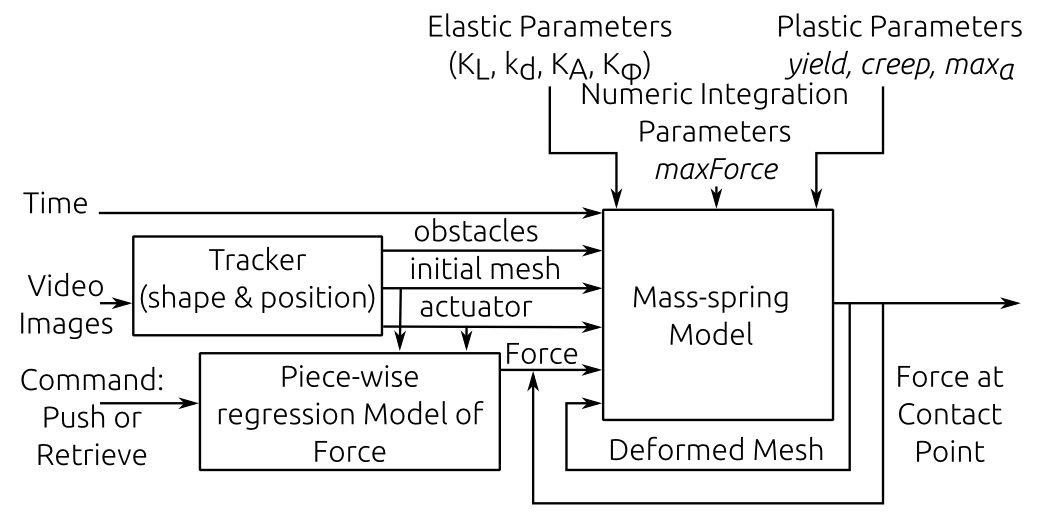
\includegraphics{arrio8}}
%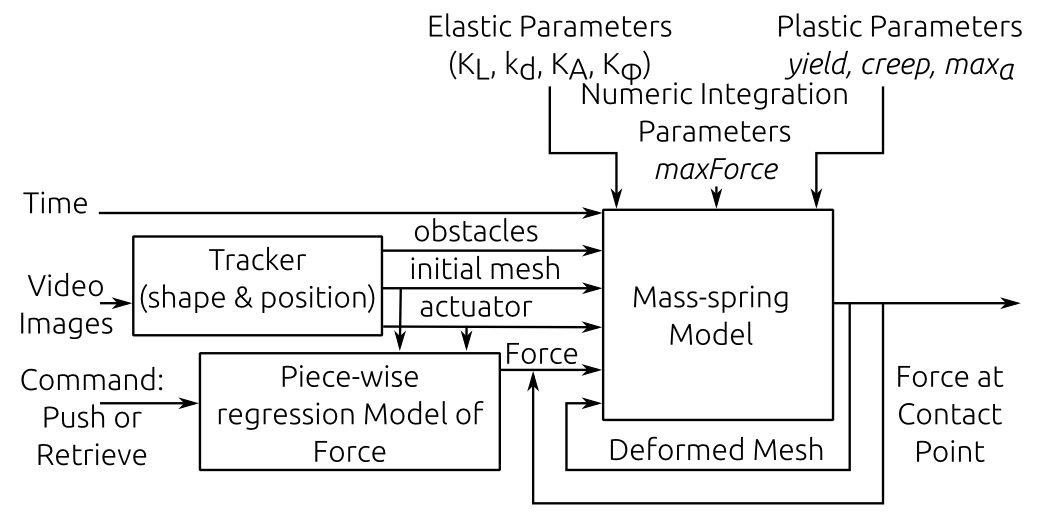
\includegraphics[width=88mm]{arrio8}
\caption{Detail of the simulation system with shape and force prediction.  The position of the actuator is extracted from the image, while the force is predicted by the piece-wise regression model (FP). This information is used by the calibrated mass-spring system (SP) to predict the shape of the object for several frames. }\label{fig:diagram}
\end{figure}

\subsection{Integration Scheme}
Sets of 24 training sessions were run, using different combinations of elasticity and plasticity terms.  For example, we used damped preservation of length only, preservation of area and angle only, or all of them together. Cases were tried including plastic deformation, and removing the collision resolution routines and the aid of geometric constraints.  For this first round of experiments three different integration schemes were used: Euler, Verlet and our customised version.  The resulting marks are summarised in \tref{tab:ischemes}.

\begin{table}[!t]
\renewcommand{\arraystretch}{1.3}
\caption{Scores of Sets of Parameters Obtained With Different Integration Schemes}
\label{tab:ischemes}
\centering
\begin{tabular}{cccc}
\hline
\bfseries Scheme & \bfseries Best & \bfseries Worst & \bfseries Average \\
\hline\hline
Euler & 0.88 $\pm$ 0.04 & 0.44 $\pm$ 0.13 & 0.75 $\pm$ 0.08 \\
Verlet & 0.76 $\pm$ 0.19 & 0.53 $\pm$ 0.18 & 0.68 $\pm$ 0.19 \\
Customised & 0.921 $\pm$ 0.008 & 0.60 $\pm$ 0.13 & 0.86 $\pm$ 0.02 \\
\hline
\multicolumn{4}{p{88mm}}{Where the mark is $\mu(F)$ as explained in \sref{sec:evaluation}.  Mean $\mu(F)$ and standard deviation across 24 training sesions are reported for the best performing models of every training session, worst model and average model.}
\end{tabular}
\end{table}

The traditional equations of movement, estimated with Euler or Verlet show big oscillations and frequently become unstable.  Verlet seems to be badly affected by the collision resolution routines and geometric aids, that drastically affect the values of velocity and acceleration.  On the other hand, the customised first degree equations suggested in \sref{sec:ischeme} produce smooth movements that more closely resemble the ground truth, thus obtaining better marks.  From this group of experiments it was also found that evolutionary learning is as efficient when considering all elastic and plastic terms, as when using only a few of them\footnote{\comment{The full list of terms is summarised at the end of \sref{sub:EvolAlg}.}}.

\subsection{Results of Automatic Parameter Calibration}
\subsubsection{Performance for the Learned Shape Prediction Model}
The performance of the genetic learning algorithm was evaluated using the customised integration scheme and the mass-spring elastic-plastic model.  At this point no prediction of the force was included, rather, the reaction forces measured with the force sensor were used. \comment{The F-score was used as fitness function. The values used for the parameters of \alref{alg:genetic} are summarised in \tref{tab:gen_params}, also the minimum and maximum limits for the values of parameters for the mass-spring model.}


\begin{table}[!t]
 \renewcommand{\arraystretch}{1.3}
 \caption{Parameters for the Genetic Algorithm}
 \label{tab:gen_params}
 \centering
\comment{
\begin{tabular}{cc}
\hline
 \bfseries Parameter & \bfseries Value/Range \\  \hline
 \multicolumn{2}{c}{Genetic Algorithm} \\ \hline
 M & 30 \\
 $\alpha = \beta = \gamma = \zeta$  & 5 \\
 $\sigma_{max}$                     & 1000.0 \\
 $\sigma_{min}$                     & 10.0 \\
 $P(s)$                             & 0.05 \\ \hline
 \multicolumn{2}{c}{Elastic Parameters } \\ \hline
 $k_d$                              & $[0.00001, 2]$ \\
 $K_L$                              & $[0.00001, 10000]$ \\
 $K_A$                              & $[0.00001, 10000]$ \\
 $K_{\varphi}$                      & $[0.00001, 100]$ \\
 $max(F)$                           & $[5, 100000]$ \\ \hline
 \multicolumn{2}{c}{Plastic Parameters } \\ \hline
 $\alpha$                           & $[0.00001, 0.9]$ \\
 $yield$                            & $[0.00001, 1.0]$ \\
 $creep$                            & $[0.00001, 1.0]$ \\ \hline
\end{tabular}

\vspace*{1em}
* Where $P(s)$ is the probability of using a special value, like $0.0$, for the spring constants.
}
\end{table}


\fref{fig:performance} shows how the quality of the simulation throughout the whole video improved with each generation.  Both graphs show that even though the enforcing of geometric constraints with additional routines may produce simulations with lower scores at the begining of the training, they perform just as well after enough generations.  These scores reflect the degree to which areas covered by the ground truth and the mesh of the simulation match; however, when looking at the videos produced, it becomes evident that simulations with additional geometric constraints succeed more in keeping the mesh flat. % Should put images? (if there is space left)

\begin{figure}[!t]
\centering
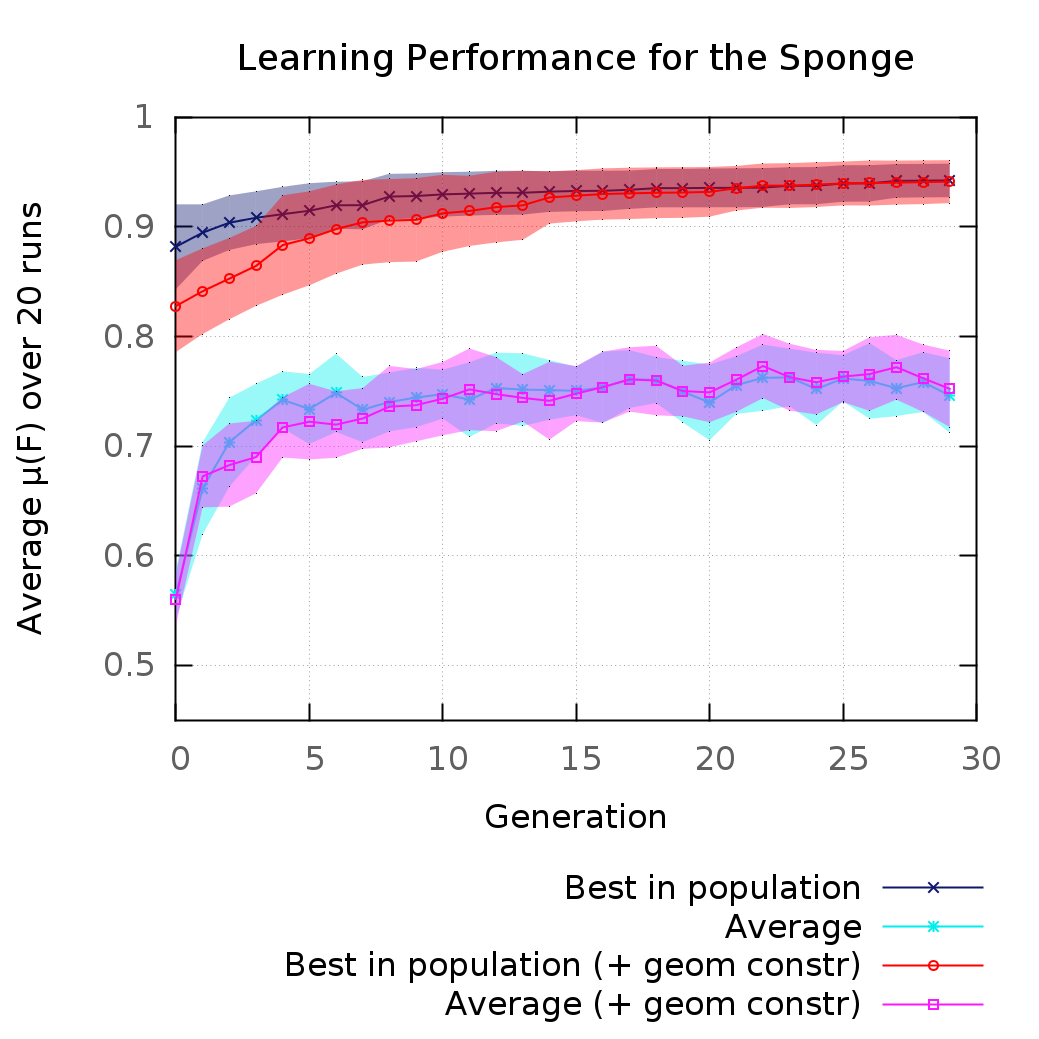
\includegraphics[width=88mm]{arrio6}
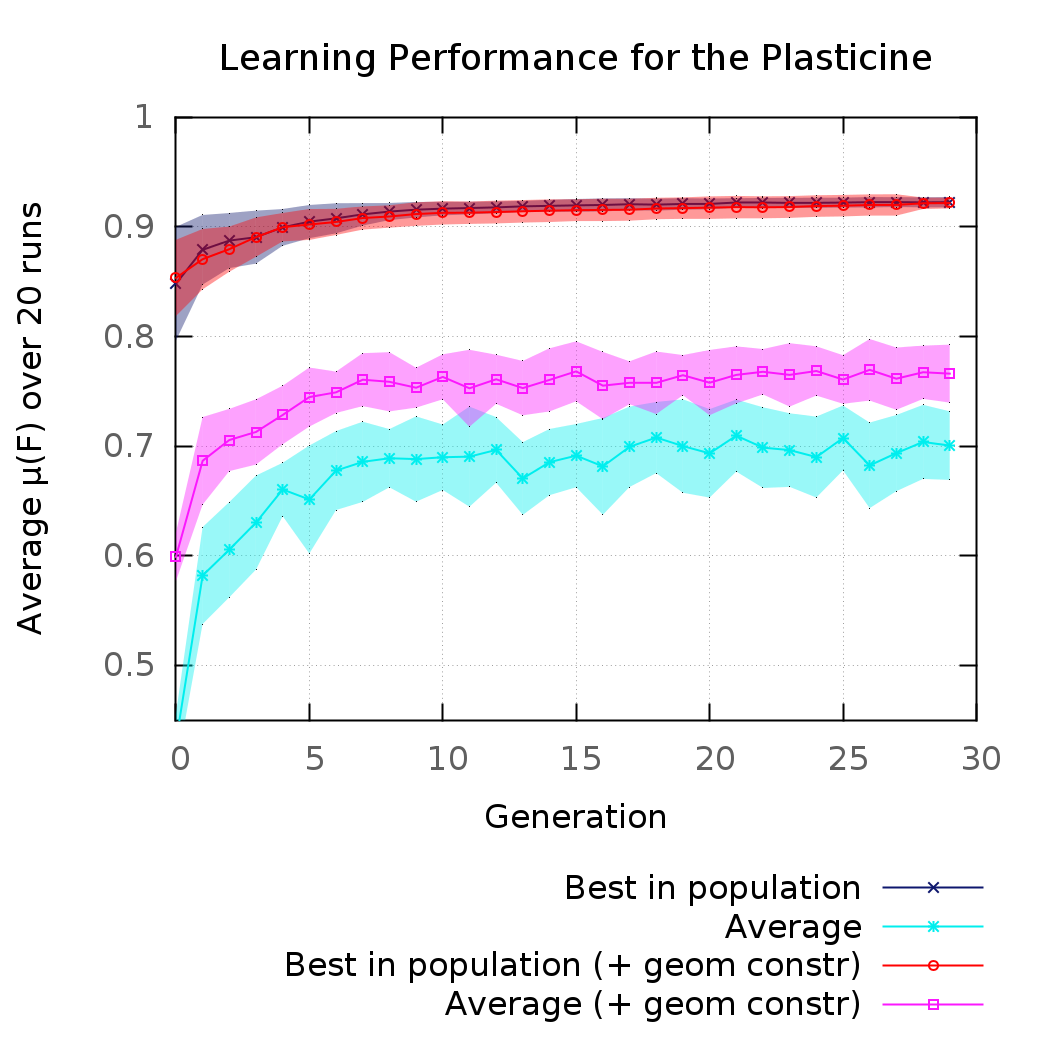
\includegraphics[width=88mm]{arrio7}
\caption{Final marks of the videos after each generation of the genetic search.  The filled areas correspond to the standard deviation $\sigma(\bar{\mu}(F))$, across 15 runs of the learning algorithm.  Using the customised integration scheme, the elastic-plastic model with all preservation terms, with and without the aid of geometric recovery routines.  The block of material was represented by a mesh of $20 \times 10$ elements.}\label{fig:performance}
\end{figure}

\subsubsection{Performance for the Learned Force Prediction Model}

\begin{figure}[!t]
\centering
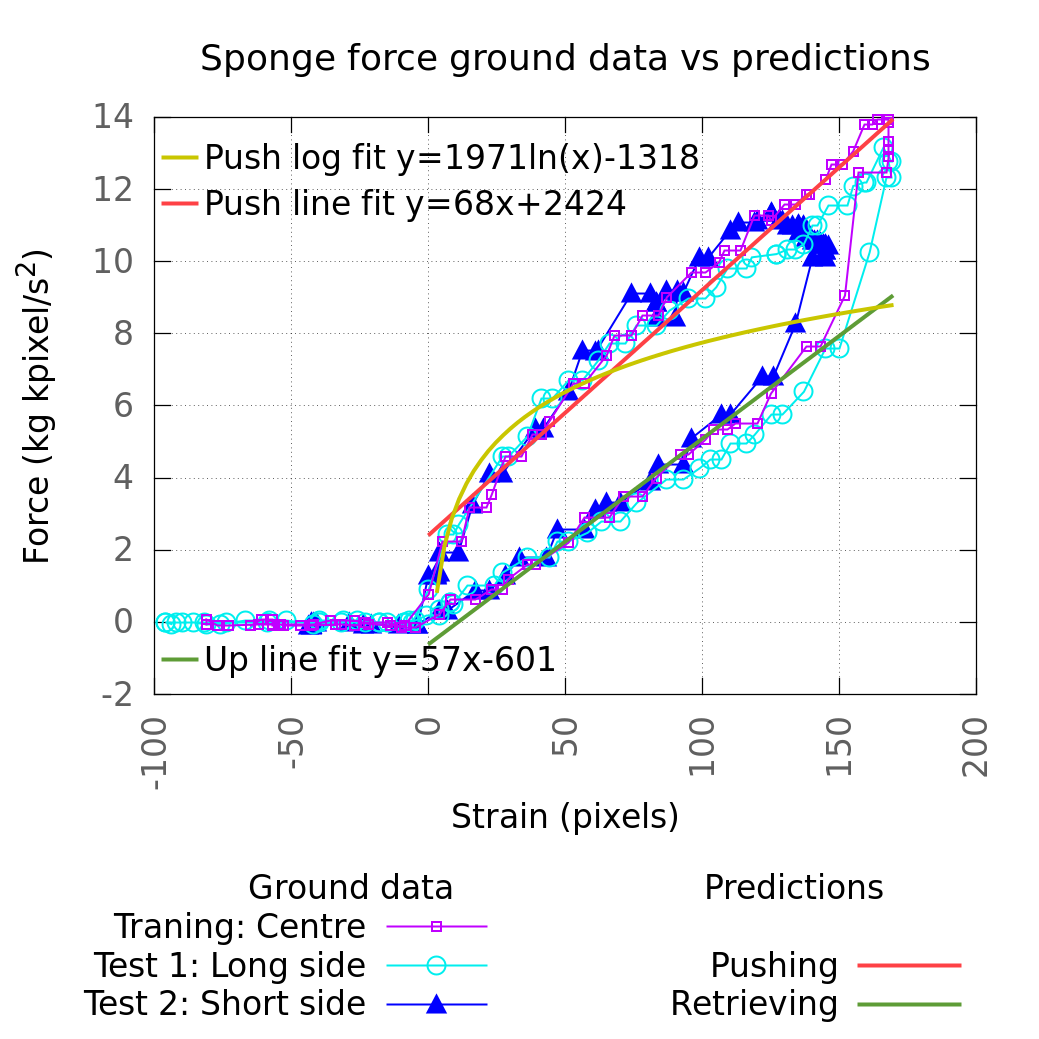
\includegraphics[width=88mm]{arrio4}
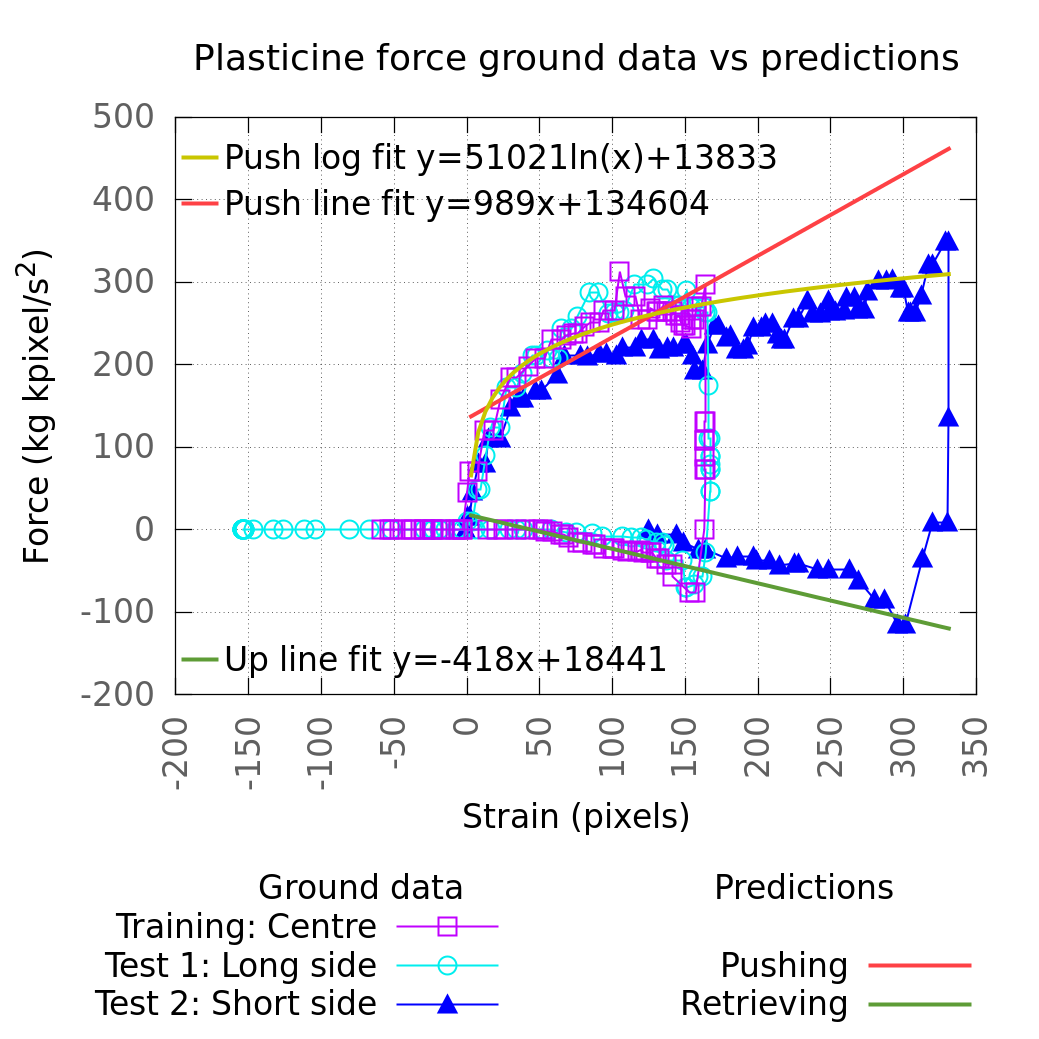
\includegraphics[width=88mm]{arrio5}
\caption{The response force during the interaction can be characterised in three phases: pushing, transition and retrieval of the finger.  A different regression curve can be used to approximate the force during the pushing and retrieving phases.  Linear and logarithmic regressions were suggested for the pushing movement and the best was chosen autonomously.  Only linear regression was used while retrieving.}\label{fig:sstrain}
\end{figure}

Using the readings of the force sensor, and associating the deformation of the material with the displacement of the robotic finger, a regression curve was fitted to the stress-strain graph for the pushing and retrieving movements.  See \fref{fig:sstrain}.  As was expected from typical stress-strain diagrams of elastic and plastic phases of materials, a linear regression is characteristic of an elastic material, while the logarithmic regression better fits a plastic material.  For the retrieving movement only a linear model was considered, since the shape deformation of the plastic material makes it harder to measure the strain from the visual information.  The curves obtained are used to approximately predict the reaction force for unknown interactions.  These forces are used for the mass-spring model as in \fref{fig:diagram}.


\subsection{Prediction}

One hundred photographs and force readings were taken every $0.17\pm0.007 s$ in average.  The mass spring model runs with an integration step $h=0.1s$, where forces that were not measured directly are interpolated.  The push down movement lasts approximately 50 frames and the retrieval movement the other 50.  The continuous lines in \fref{fig:sstrain} show the predicted forces, given the amount of compression of the material (strain), while the point-lines show the actual readings.  \fref{fig:simulation_sponge} and \fref{fig:simulation_plasticine} show the actual shapes predicted by the combined FP and SP model.

\begin{figure*}[!t]
\centering
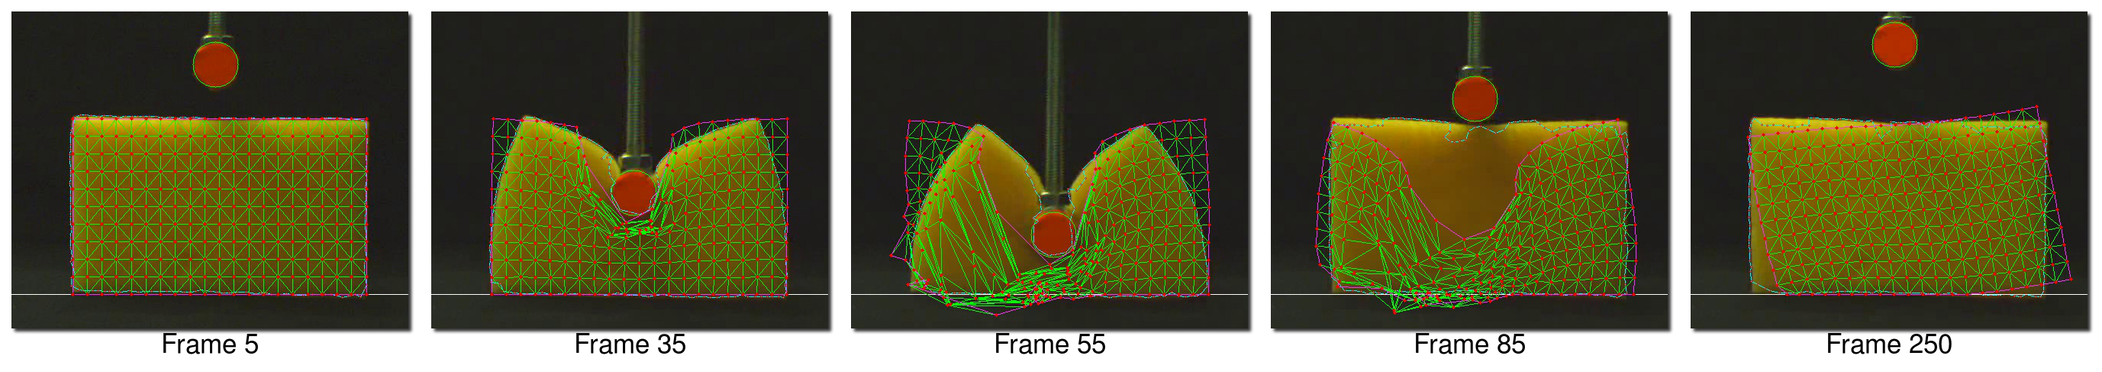
\includegraphics[width=178mm]{arrio9}
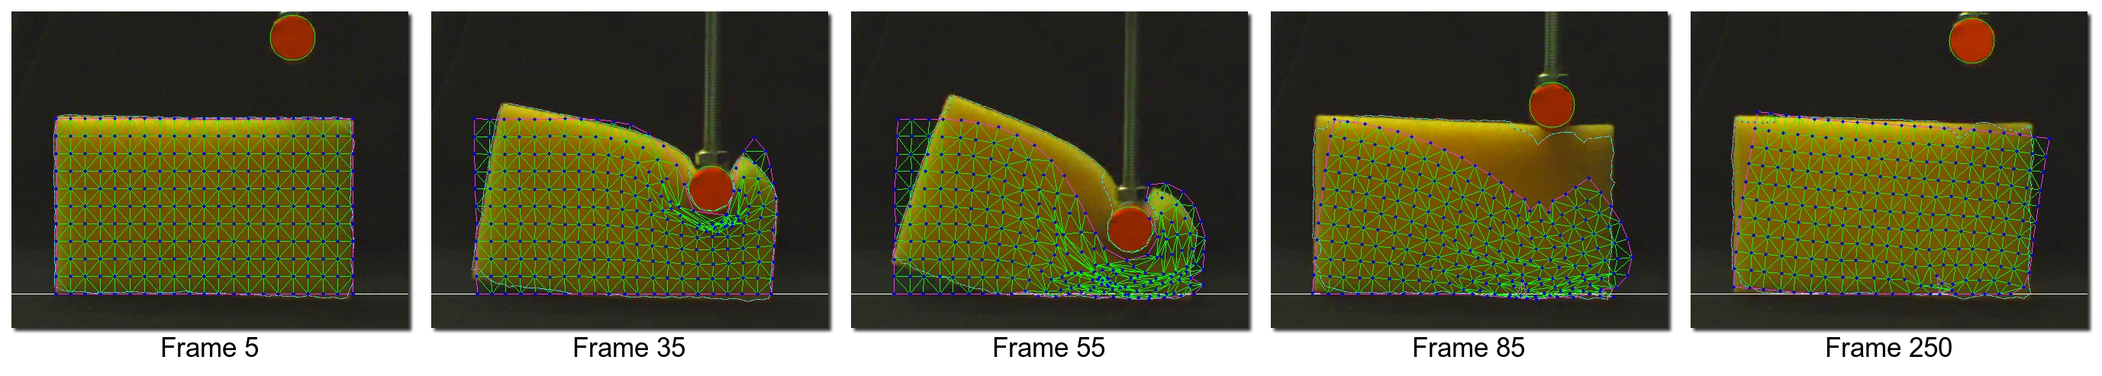
\includegraphics[width=178mm]{arrio10}
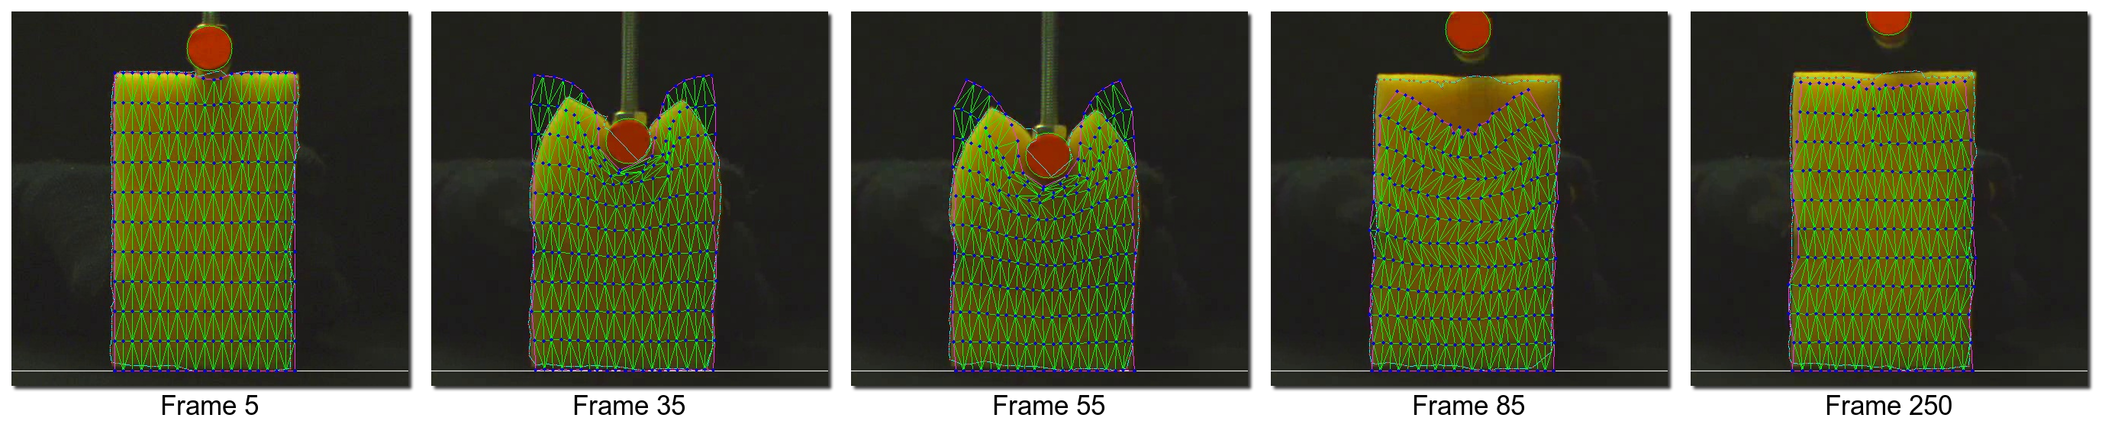
\includegraphics[width=178mm]{arrio11}
\caption{Simulation of the sponge obtained with parameters $k_L=3034.48, k_d=0.000237, k_A=103.568 k_{\phi}=66.774, max\_Force=1218.81, yield=0.000434973, creep=0.00890343, max\_\alpha=0.45204$.  Using the customised integration scheme, the elastic-plastic model with all preservation terms, with the aid of geometric recovery routines and collision detection with the finger.  The block of material was represented by a mesh of $20 \times 10$ elements. Top: Training. Middle: Test 1. Bottom: Test 2}\label{fig:simulation_sponge}
\end{figure*}

\begin{figure*}[!t]
\centering
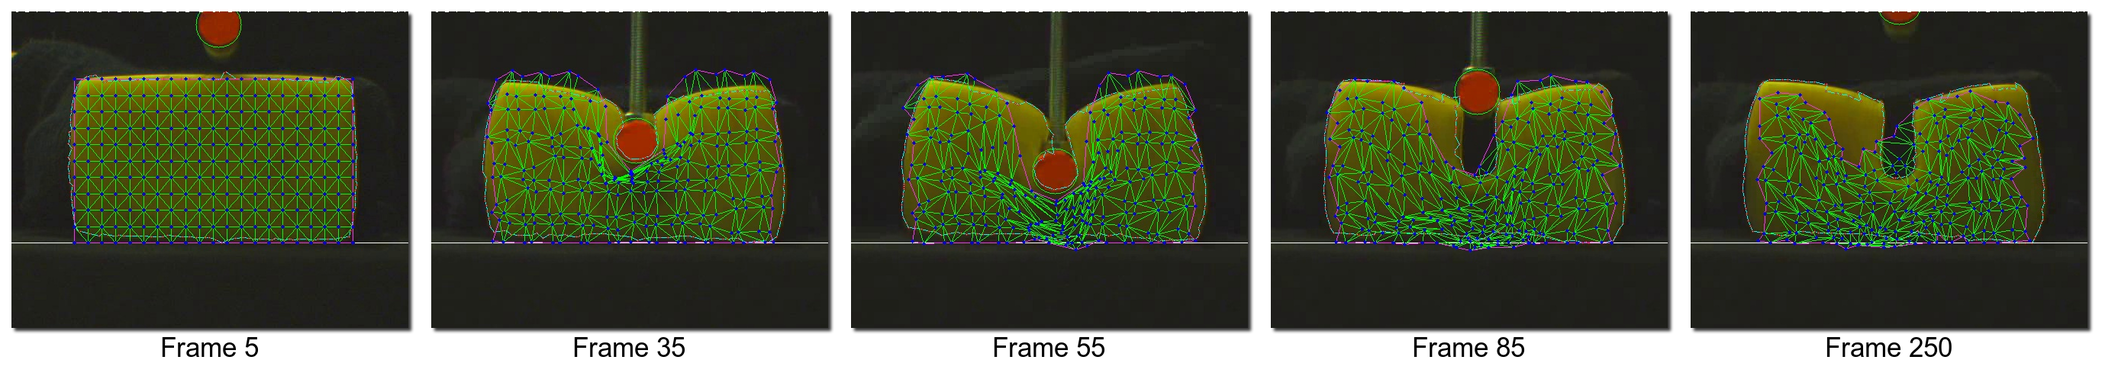
\includegraphics[width=178mm]{arrio12}
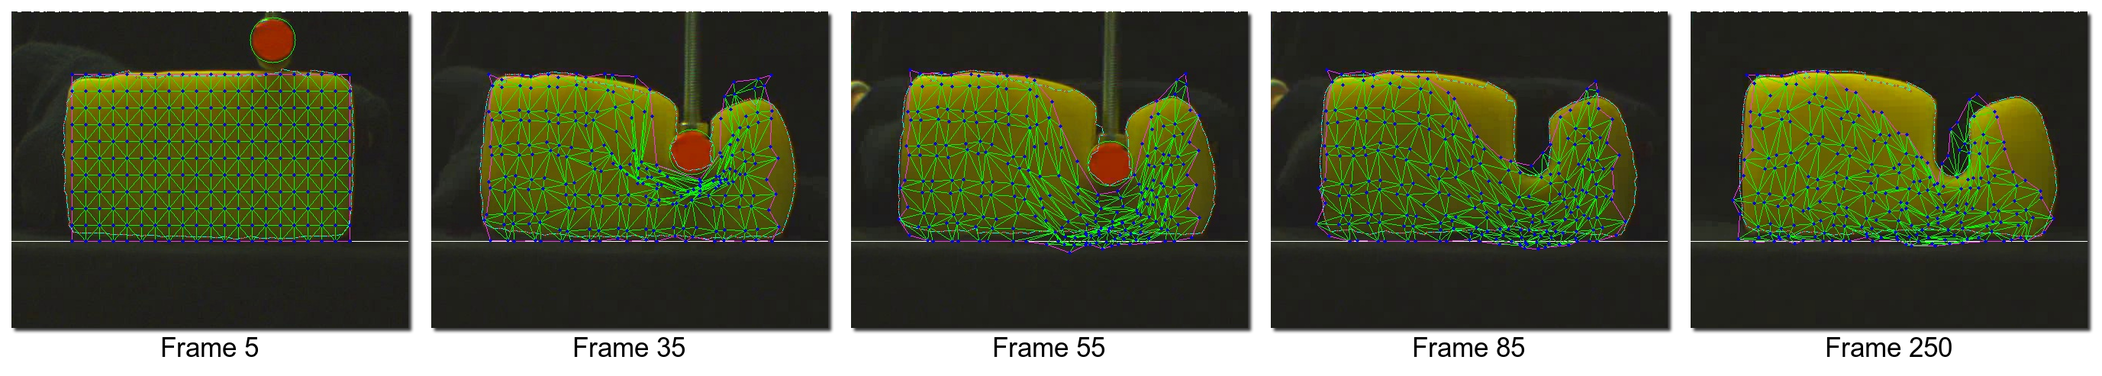
\includegraphics[width=178mm]{arrio13}
%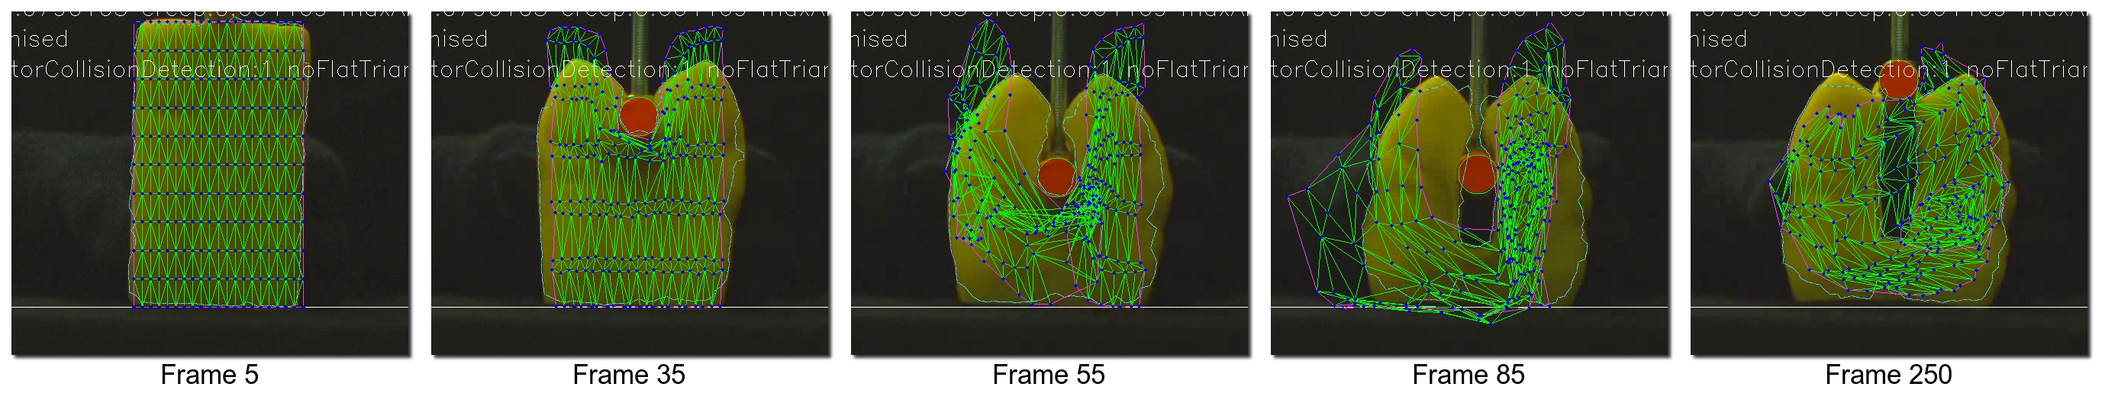
\includegraphics[width=178mm]{arrio14}
\caption{Simulation of the plasticine obtained with parameters $k_L=642.328, k_d=0.562201, k_A=29.2776 k_{\phi}=72.6202, max\_Force=765.912, yield=0.0790105, creep=0.664469, max\_\alpha=0.48842$.  Using the customised integration scheme, the elastic-plastic model with all preservation terms, with the aid of geometric recovery routines and collision detection with the finger.  The block of material was represented by a mesh of $20 \times 10$ elements. Top: Training. Middle: Test 1. Bottom: Test 2}\label{fig:simulation_plasticine}
\end{figure*}

\begin{figure*}[!t]
\centering
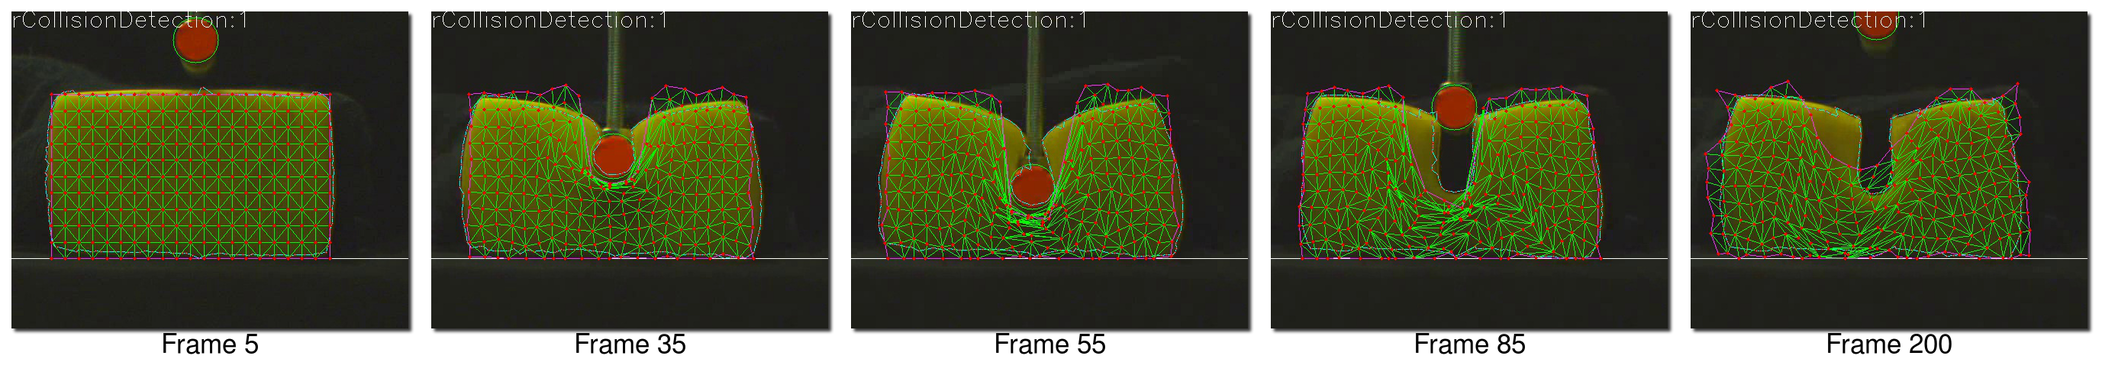
\includegraphics[width=178mm]{arrio16}
\caption{Simulation of the plasticine obtained with parameters $k_L=0, k_d=0, k_A=28202.1 k_{\phi}=34.5491, max\_Force=780.825, yield=0.772727, creep=0.67466, max\_\alpha=0.656572$.  Using the customised integration scheme, the elastic-plastic model with some preservation terms, furtherly tuned by hand,  with the aid of geometric recovery routines with the finger.  The block of material was represented by a mesh of $20 \times 10$ elements.}\label{fig:simulation_plasticine_hand}
\end{figure*}

\comment{We also compared the generalisation capabilities of our model against the system proposed in \cite{Cretu2012}.  This system uses a Growing Neural Gas (GNG) Network to calibrate a colour segmentation algorithm.  We couldn't use the HSV space, as suggested by Cretu, because our videos have lots of shadows which produce holes inside the material regions which cause problems in further stages.  We obtained better results for GNGN with the Luv color space.  Note that, even though we used the HSV space in our tracking algorithm, this didn't have the same problems because the nodes of our linear snake search for nearby edges and are not affected by shadows in the middle of the object or temporary failures in detecting an edge.  Another GNG network is used to select the control points adequate for approximating the contour in the first frame.  Later, Cretu et al. used a Neural Gas (NG) algorithm to adjust that fixed number of control points to the contour of the material at every frame.  Using the coordinates of the finger, the sensed force and the coordinates of those control points through time, they train a Feedforward Neural Network (FFNN) to predict the contour of the material given the position of the finger and sensed force.  We reproduced those steps and their training method on our training video.  However, when we tried to test the generalisation capabilities of their method to new pushing actions, the weakness of the FFNN method became evident: it became tied to the specific location and type of interaction it was trained with, while our physics based model had no problem making predictions for new pushing actions.  The results with the GNGN method can be seen in \fref{fig:cretu_prediction}.

%Since the videos with the plasticine have even greater shadows it was not posible to use their tracking algorithm on them.  However, even if we could change that algorithm, we would expect the system to have the same problems and predict the deformation at the middle of the material even if is being pushed somewhere else. 
}

\begin{figure}[!t]
\centering
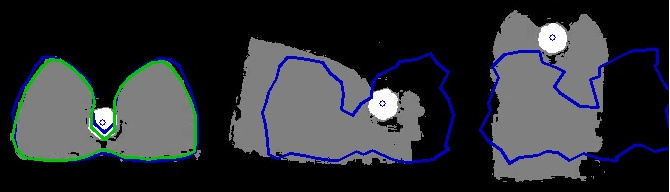
\includegraphics[width=3.5in]{sponge__result.jpg}
\caption{Neural network approach fits quite well the training data set, but can not generalise to new pushing actions.  The red line shows the border used as ground truth in the training set, while yellow lines show prediction from the FFNN.}\label{fig:cretu_prediction}
\end{figure}
\begin{figure}[!t]
\centering
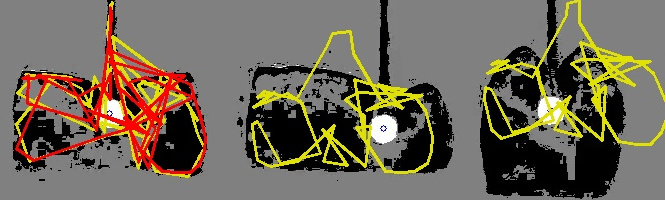
\includegraphics[width=3.5in]{plasticine__result.jpg}
\caption{GNG segmentation didn't work with a shadowed material (video of plasticine). This image shows the segmentation results previous to the application the median filter, which was applied to perform tracking.  Results also do not generalise to unseen pushing actions.  The red line shows the border used as ground truth in the training set, while yellow lines show prediction from the FFNN.}\label{fig:cretu_prediction}
\end{figure}

\subsection{Classification}

The mass-spring models calibrated for the prediction task were used to classify materials through recognition of their behaviour, even when the objects where pushed and deformed at novel locations.  The models make predictions as if the material of the object was known.  The model that makes the best predictions indicates which type of object is being observed.  There are two criteria for selecting an object/material for the video being shown to the system:

\begin{enumerate}
 \item Per frame: a material is selected for each frame of the interaction according to whichever model made the best prediction for that particular frame, according to the F-score. This test was performed for every frame of the six videos, where the robot finger pushes the block of material.

 \item Global: The system makes a vote about which material the object was made of, for the whole duration of the video, by making use of a weighted score. The difference in the F-score is added for all frames.  Frames where the distinction is more noticeable will receive a greater weight.
\end{enumerate}



\section{Discussion}
\label{sec:discussion}
We note the following points about the results and the method in general.
\subsection{The Learning Method}
Even though the evolutionary algorithm allowed for a uniform exploration of the logarithmic space of parameters, it failed to find the optimal solution.  Better simulations have been obtained by hand tuning some of the \comment{best sets of parameters obtained by the genetic algorithn.  This is not due to an error of the search algorithm, but due to a difference between what humans visually qualify as a good solution and what the evaluation function does.  For example: humans would prefer the solution shown in \fref{fig:simulation_plasticine_hand}, because this model of the plasticine does not tend to recover its shape, as the one selected by the computer does.  However, the f-score of the solution chosen by the computer is better.  The similarity between the sensed force and the forces that the mass-particles produce on the finger could be added as a second criteria to evaluate the models.  Even though we found that the automatic calibration procedure sometimes produces models were this difference is small, we have left for future work the addition of this criterion to the evaluation function.}

\subsection{Using Additional Geometric Constraints}
Adding extra routines to enforce the planarity of the mesh had good aesthetic results, however that did not reflect much on the mark for the best videos of each generation during training.   Also, when attempting to model the plastic material, the geometric constraints provoked a much larger effect caused by the plasticity term, even if its corresponding constant was small.  As a consequence the plastic material also recovered its original shape after some extra frames.  It has been seen that, if the constant for linear preservation is set to zero, the problem disappears.  Even if the automatic calibration selects these extreme values with probability $\epsilon>0$, in an attempt to reproduce this finding, their derivatives obtained after applying gaussian noise to their parameters obtain better marks, even though they eventually recover their shapes, and get selected in a better position for the next generation.  We hypothesise that humans give greater weight to specific aspects of the simulation, for example: to the beginning, to the instant of greatest deformation and to the final shape.  Meanwhile, the evaluation function gives the same weight to all frames in the sequence.  It is possible to use the force learning algorithm and the commands given to the robot (push/retrieve) to detect these points, since they are correlated with discontinuities in these other modalities.  Future work will evaluate the impact of these modifications on the evaluation function.

\subsection{Training With Collision Resolution with the Finger vs. Without}
It was found that the overall score of the best simulations was similar in both cases, since only geometric similarities are under consideration.  However, there was a noticeable difference in the rate of success for the classification problem.  If no collision detection with the finger is used during training, the springs react only to the forces and, if the spring coefficients are not adequate, the shape of the mesh will be very different from the shape of the ground truth.

On the other hand, if collision detection is used, the geometric constraints strongly favour a correct configuration of the mesh in the vicinity of the actuator, even though the springs did not react properly.  For subsequent frames, it is more likely, when using collision detection, that the neighbours will succeed in propagating the deformation to the rest of the material, thus producing better simulations than without it.  However, this lessens the effectiveness of the mass-spring model in distinguishing the materials.

\subsection{Classification}

\begin{table}[!t]
\renewcommand{\arraystretch}{1.3}
\caption{Classification per Frame}
\label{tab:classperframe}
\centering
\begin{tabular}{ccccccccc}
\hline
 & & \multicolumn{3}{c}{\bfseries Sponge} & & \multicolumn{3}{c}{\bfseries Plasticine} \\
Data Set & & TP & FN & Precision & & TP & FN & Precision\\
\hline\hline
 \multicolumn{9}{c}{Trained with forces on vertices and no collision resolution.} \\
\hline
   training & & 167 & 132 & 0.56 & & 186 & 113 & 0.62 \\
   test1 & & 167 & 132 & 0.56 & & 271 & 28 & 0.91 \\
   test2 & & 242 & 57 & 0.81 & & 289 & 10 & 0.97 \\ 
\hline
\multicolumn{9}{p{0.9\columnwidth}}{\begin{footnotesize}\comment{* TP and FN are measured in terms of numbers of frames. TP + FN = 299.  The final class assigned according to the performance of the models' predictions across the whole video. See text for details.} \end{footnotesize}}
\end{tabular}
\end{table}


% \begin{table}[!t]
% \renewcommand{\arraystretch}{1.3}
% \caption{Classification per Frame}
% \label{tab:classperframe}
% \centering
% \begin{tabular}{ccccccccc}
% \hline
%  & & \multicolumn{4}{c}{\bfseries Sponge} \\
% Data Set & & TP & FN & TN & FP & Precision \\
% \hline\hline
%  \multicolumn{9}{c}{Trained with forces on vertices and no collision resolution.} \\
% \hline
%    training & & 167 & 132 & & & 0.56  \\
%    test1 & & 167 & 132 & & & 0.56  \\
%    test2 & & 242 & 57 & & & 0.81 \\ 
% \hline
% %\multicolumn{7}{p{68mm}}{\begin{footnotesize}* TP and FN measured in number of frames.  Final class assigned according to the performance of the models' predictions across the whole video. \end{footnotesize}}
% \end{tabular}
% 
% \vspace*{1em}
% \begin{tabular}{ccccccccc}
% \hline
%  & & \multicolumn{4}{c}{\bfseries Plasticine} \\
% Data Set & & TP & FN & TN & FP & Precision\\
% \hline\hline
%  \multicolumn{9}{c}{Trained with forces on vertices and no collision resolution.} \\
% \hline
%    training & & 186 & 113 & & & 0.62 \\
%    test1 & & 271 & 28 & & & 0.91 \\
%    test2 & & 289 & 10 & & & 0.97 \\ 
% \hline
% %\multicolumn{7}{p{68mm}}{\begin{footnotesize}* TP and FN measured in number of frames.  Final class assigned according to the performance of the models' predictions across the whole video. \end{footnotesize}}
% \end{tabular}
% \end{table}

\comment{
\tref{tab:classperframe} shows the results for the classification task, frame by frame for each video.  When the sponge model performed better for a frame of the sponge video it is marked as a true positive (TP), when plasticine does better it is marked as a false negative (FN) ---since it didn't recognize it as a sponge.  The analogous process is used for the plasticine. The total TP+FN=299 which is the total frames per movie. The overall classification for a movie can be determined by whether TP > FN or vice versa. Using this rule gives a perfect classification of the six movies.

It should be noted that, in some of the experiments, the performance of classification for the sponge on the training and test1 sets are the same.  We interpret that the mass-spring physics based model generalizes naturally when the force/deformation conditions are similar, even if the place for pushing is different.  Between pushing in the middle and pushing closer to the border the qualitative behaviour of the elastic material was no so different for these models; unlike the data from the third set, where the distribution of mass and maximum force/deformation is more different from the ones seen on the training set of the model.  It is interesting to confirm that the difference in predictions between the models is bigger here, resulting in better classification.

It is also notable that, when modeling the sponge, the parameters for the plasticine were close in performance to the parameters for sponge (thus causing more problems to establish a good classification), the opposite does not happen.  That is, the parameters for the sponge are not good at modeling the plasticine on the test sets, thus yielding better results at the classification task.  This could happen because the plastic behaviour (that is, the permanent deformation of a spring) gets activated with stronger forces after the $yield$ limit is reached, which only appear when pushing the plasticine.  With the small forces fed back by the sponge, the model for the plasticine does not reach its range of plastic behaviour and thus the big differences in behaviour are not manifest.
}

The best results for classification with the mass-spring model are obtained when the training of the models uses only forces to displace the nodes in the mass-spring model\footnote{Case 2 in \sref{sec:manysteps}}, but the combination of force readings and collision resolution is used during classification\footnote{Case 3 in \sref{sec:manysteps}}.  This finding agrees with the fact that the objects are more distinguishable from the data obtained from the force sensor, than from the visual data.  The fact that the spring constants must respond to the applied forces during the training and not only to the visual appearance is reflected in a better differentiation of the behaviour of the models.  When the calibration is more sensitive to the constants of the springs, it is more robust for novel interactions, therefore the difference in quality of the predictions is a better indicator of which material is being used.

\subsection{Conclusions}
In summary, we have presented a framework and specific algorithms for off-line learning of the sensorimotor contingencies for the deformable behaviour of objects under robot pushing. We have developed an approach that learns/calibrates the parameters of two contingencies that are sequenced, one for kinematic motion to force (FP) and the other for force to deformation (SP). By sequencing these we obtained a compound contingency that predicts deformation given motion. The main properties of the model are as follows. First, the parameters for the model components were learned from data from real objects under robotic manipulation. Second, we have attempted the automatic calibration of a simulation of plasticity. \comment{If a new material were added, provided it were elastic or plastic, it would be possible to calibrate a model for that material, independent of the existing calibrated models.} Third, we use regression to predict the reaction forces in the force prediction model. Fourth, we include a new energy term for the preservation of angles in a mass-spring model of shape deformation. Fifth, we employ a regularization algorithm for a linear snake, that increases or decreases the number of its control points, according to the level of detail required to represent the deformed object. Sixth, we provide a detailed evaluation of the dynamic simulation, instead of only during its stable states as in previous work. Finally we showed the application of the learned prediction models to the problem of classifying deformable materials.

There is considerable future work to be done. The first extension is due to the fact that we restricted the deformation model to 2D, and this can easily revert to the 3D meshes as used in Teschner's original work. The second issue is to explore new methods for the learning phase. The current search procedure doesn't always find good solutions for the plastic deformation model. A third extension is to extend the fairly trivial visual system to initialise mass-spring models for objects of abitrary shape. We propose using a Voronoi triangulation rather than a grid. But a more basic problem is that mass-spring models restrict the range of deformations that can be modelled. While the framework presented here is promising, we regard the actual deformation model representation as an open research problem. \comment{Finally, all the work here is for off-line learning, from a carefully chosen viewpoint. The issue of online learning of these representations, including how to explore so as to learn, is an open issue.}

% if have a single appendix:
%\appendix[Proof of the Zonklar Equations]
% or
%\appendix  % for no appendix heading
% do not use \section anymore after \appendix, only \section*
% is possibly needed

% use appendices with more than one appendix
% then use \section to start each appendix
% you must declare a \section before using any
% \subsection or using \label (\appendices by itself
% starts a section numbered zero.)
%
\appendix[Forces Derived from Preservation Constraints]
\label{ap:formulas}

\subsubsection{Preservation of Length}

Substituting \eref{eq:clength} in \eref{eq:Fdamping}, after some manipulation we get:
\begin{align}
 \vec{F}^i_D(p_i,p_j,v_i,v_j) &= \dfrac{k_L}{D_0^2} \left( |\vec{p}_j-\vec{p}_i|-D_0 \right) \dfrac{\vec{p}_j-\vec{p}_i}{|\vec{p}_j-\vec{p}_i|}  + \nonumber \\
 & \dfrac{k_d}{D_0^2}\left( \dfrac{\vec{p}_j-\vec{p}_i}{|\vec{p}_j-\vec{p}_i|} \cdot (\vec{v}_j-\vec{v}_i) \right) \dfrac{\vec{p}_j-\vec{p}_i}{|\vec{p}_j-\vec{p}_i|} \label{eq:FDlength}
\end{align}
where $k_L$ is the linear spring constant and $k_d$ the damping constant.

\subsubsection{Preservation of Area}

The force $\vec{F}^i_A$ is derived as follows: 
\begin{align}
 C &= \frac{\frac{1}{2}|(\vec{p}_j-\vec{p}_i)\times(\vec{p}_k-\vec{p}_i)|-A_0}{A_0} \\
 A &= \frac{1}{2}|(\vec{p}_j-\vec{p}_i)\times(\vec{p}_k-\vec{p}_i)|, \\
 \vec{F}^i_A(p_i,p_j,p_k) &= -\frac{k_A}{2A_0^2} \left( A-A_0 \right) \nonumber \\
 & \frac{(\vec{p}_j-\vec{p}_i)\times(\vec{p}_k-\vec{p}_i)}{|(\vec{p}_j-\vec{p}_i)\times(\vec{p}_k-\vec{p}_i)|} [\vec{1} \times (\vec{p}_j-\vec{p}_k)] \label{eq:area_force}
\end{align}
where $A_0$ is the initial area of the triangle and $k_A$ the proportionality constant.

It is possible to rewrite \eref{eq:area_force} in a more geometrically intuitive manner by rewriting the direction of the gradient according to Morris' geometric derivation \cite{Morris2008}, but keeping the area normalisation constant\footnote{This substitution is valid because both are expressions for the gradients of the area of the triangle formed by the three verticies.}.  It becomes evident that the forces pull along the heights of the triangles [\fref{fig:forces}(b)].  Then the magnitude of the force is given by:
\begin{equation}
 \lVert \vec{F} \rVert_A(\vec{p}_i)= \frac{\frac{1}{2}|(\vec{p}_j-\vec{p}_i)\times(\vec{p}_k-\vec{p}_i)|-A_0}{A_0^2}
\end{equation}

While the rest becomes:
\begin{align}
 \vec{F}_A(\vec{p}_i) & = k_A \cdot \lVert \vec{F} \rVert_A(\vec{p}_i) \cdot forcedir_A(\vec{p}_i) \nonumber \\
 forcedir_A(\vec{p}_i) & = \dfrac{\vec{F}_A(\vec{p}_i)}{|\vec{F}_A(\vec{p}_i)|} = \dfrac{\nabla A(\vec{p}_i)}{|\nabla A(\vec{p}_i)|} \nonumber \\
 \nabla A(\vec{p}_i) & = (\vec{p}_i-\vec{p}_j)- \nonumber \\
 & \left( (\vec{p}_k-\vec{p}_j) \cdot \dfrac{(\vec{p}_k-\vec{p}_j) \cdot (\vec{p}_i-\vec{p}_j)}{(\vec{p}_k-\vec{p}_j) \cdot (\vec{p}_k-\vec{p}_j)} \right)
\end{align}

\subsubsection{Preservation of Angles}

The force is derived from:  %An additional line in the code also forces an inverted angle to recover its original orientation.
\begin{align}
 F_\varphi(p_i) & = k_\varphi(\varphi - \varphi_0)\dfrac{\partial \varphi}{\partial p_i} \\
 \dfrac{\partial \varphi}{\partial p_i} & = \dfrac{\partial}{\partial p_i} arccos \left(\frac{(\vec{p}_j-\vec{p}_i)\cdot(\vec{p}_k-\vec{p}_i)}{\left\|\vec{p}_j-\vec{p}_i\right\|\left\|\vec{p}_k-\vec{p}_i\right\|}\right) \displaybreak[0] \\
\end{align}

The force is:
\begin{align}
 F_\varphi(p_i) & = k_\varphi(\varphi - \varphi_0)\dfrac{\partial \varphi}{\partial p_i} \\
 \dfrac{\partial \varphi}{\partial p_i}(p_i) & =
    \dfrac{1}{d_{ji}d_{ki}\sqrt{1-\left[\dfrac{pp}{(d_{ji}) (d_{ki})}\right]^2}} \nonumber \\
 & \left\{\left[1-\dfrac{pp}{d_{ki}^2}\right](p_k-p_i)+\left[1-\dfrac{pp}{d_{ji}^2}\right](p_j-p_i) \right\} \nonumber \\
 pp(p_i) & =(p_j-p_i)\cdot(p_k-p_i) \nonumber \\
 d_{ji}(p_i) & = \left\| p_j-p_i \right\| \nonumber \\
 d_{ki}(p_i) & = \left\| p_k-p_i \right\|
\end{align}

% \appendices

% you can choose not to have a title for an appendix
% if you want by leaving the argument blank
% \section{}
% Appendix two text goes here.


% use section* for acknowledgement
\section*{Acknowledgment}

We gratefully acknowledge funding from the PhD Scholarship program of CONACYT, Mexico and from the European Community's FP7 program, under grant agreements 215181 CogX, and 600918 PaCMan.


% Can use something like this to put references on a page
% by themselves when using endfloat and the captionsoff option.
\ifCLASSOPTIONcaptionsoff
  \newpage
\fi


\balance

% trigger a \newpage just before the given reference
% number - used to balance the columns on the last page
% adjust value as needed - may need to be readjusted if
% the document is modified later
%\IEEEtriggeratref{15}
% The "triggered" command can be changed if desired:
%\IEEEtriggercmd{\enlargethispage{-5in}}

% references section

% can use a bibliography generated by BibTeX as a .bbl file
% BibTeX documentation can be easily obtained at:
% http://www.ctan.org/tex-archive/biblio/bibtex/contrib/doc/
% The IEEEtran BibTeX style support page is at:
% http://www.michaelshell.org/tex/ieeetran/bibtex/
%\bibliographystyle{IEEEtran}
\bibliographystyle{IEEEtranS}
% argument is your BibTeX string definitions and bibliography database(s)
\bibliography{twostagedo,jlw}


%
% <OR> manually copy in the resultant .bbl file
% set second argument of \begin to the number of references
% (used to reserve space for the reference number labels box)
% \begin{thebibliography}{1}
% 
% \bibitem{IEEEhowto:kopka}
% H.~Kopka and P.~W. Daly, \emph{A Guide to \LaTeX}, 3rd~ed.\hskip 1em plus
%   0.5em minus 0.4em\relax Harlow, England: Addison-Wesley, 1999.
% 
% \end{thebibliography}

% biography section
% 
% If you have an EPS/PDF photo (graphicx package needed) extra braces are
% needed around the contents of the optional argument to biography to prevent
% the LaTeX parser from getting confused when it sees the complicated
% \includegraphics command within an optional argument. (You could create
% your own custom macro containing the \includegraphics command to make things
% simpler here.)
%\begin{IEEEbiography}[{\includegraphics[width=1in,height=1.25in,clip,keepaspectratio]{mshell}}]{Michael Shell}
% or if you just want to reserve a space for a photo:

\begin{IEEEbiography}[{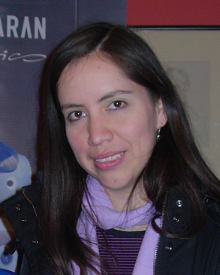
\includegraphics[width=1in,height=1.2in,clip,keepaspectratio]{arrio}}]{Veronica E. Arriola-Rios}
  has recently obtained her PhD in Computer Science from the University of Birmingham.
  She works as full time lecturer at the National Autonomous University of Mexico (UNAM).
  Veronica holds undergraduate degrees in Physics and Computer Science, and a masters degree in Computer Sciences, in the area of Computer Graphics and Virtual Environments.
  Her research interests include artificial inteligence, cognitive robotics and natural cognition.
\end{IEEEbiography}

\begin{IEEEbiography}[{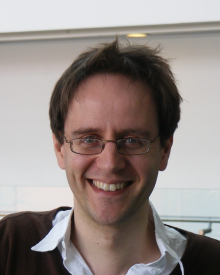
\includegraphics[width=1in,height=1.2in,clip,keepaspectratio]{wyatt}}]{Jeremy L. Wyatt} is Professor of Robotics
  and Artificial Intelligence at the University of Birmingham. He
  obtained a BA in Theology from the University of Bristol, an MSc in
  Knowledge Based Systems from the University of Sussex, and his
  Ph.D. in Artificial Intelligence from the University of Edinburgh in
  1997. He was a Leverhulme Fellow from 2006-8. He has won two best paper prizes, published more than 100 refereed articles, led two international research projects on robot planning and learning (CogX) and robot manipulation (PaCMan), and edited three books. His interests
  include machine learning, planning, architectures, vision, mobile robotics and robot manipulation.
\end{IEEEbiography}

\vfill
% insert where needed to balance the two columns on the last page with
% biographies

% You can push biographies down or up by placing
% a \vfill before or after them. The appropriate
% use of \vfill depends on what kind of text is
% on the last page and whether or not the columns
% are being equalized.

% Can be used to pull up biographies so that the bottom of the last one
% is flush with the other column.
%\enlargethispage{-5in}

% that's all folks
\end{document}
